\documentclass{mini}

\usepackage[utf8]{inputenc}
\usepackage{color}
\usepackage{xcolor}
\usepackage{colortbl}
\usepackage{tikz}
\usepackage{tikz-qtree}
\usepackage{caption}
\usepackage{subcaption}
\usepackage{multirow}
\usepackage{tabularx}
\usepackage{lscape}
\usepackage{verbatim}
\usepackage{algorithm}
\usepackage{algorithmic}
%\usepackage[noend]{algpseudocode}
\usepackage{caption}


\makeatletter
\renewcommand{\ALG@name}{Algorytm}
\makeatother

\setlength{\extrarowheight}{3pt}
\usetikzlibrary{calc, shapes, backgrounds, arrows, positioning, calc}

\definecolor{mojkolor}{rgb}{0.99, 1, 0.99}
\newenvironment{dow}{\textbf{\textit{Dowód}}}{\begin{flushright} $\blacksquare$ \end{flushright}}
\newcommand{\argmin}{\arg\!\min}
\newcommand{\argmax}{\arg\!\max}

\newlength\myindent
\setlength\myindent{2em}
\newcommand\bindent{%
  \begingroup
  \setlength{\itemindent}{\myindent}
  \addtolength{\algorithmicindent}{\myindent}
}
\newcommand\eindent{\endgroup}

%------------------------------------------------------------------------------%
\title{Statystyczne metody regresji porządkowej}
\titleaux{Statistical methods for ordinal regression}
\author{Marta Sommer}
\tytsupervisor{prof. nzw. dr hab.}
\supervisor{Przemysław Grzegorzewski}
\type{magisters}
\discipline{matematyka}
\monthyear{grudzień 2015}
\date{\today}
\album{237503}
%------------------------------------------------------------------------------%

\begin{document}

\maketitle
\tableofcontents

\chapter*{Streszczenie}

Uczenie maszynowe często natrafia na problem klasyfikacji wieloklasowej (ang. \textit{multinomial regression}), w której zmienna odpowiedzi jest w pewien naturalny sposób uporządkowana. Mamy wtedy do czynienia z tzw. regresją porządkową (ang. \textit{ordinal regression}). 

Głównym celem mojej pracy jest zebranie, omówienie i porównanie dostępnych w literaturze metod modelowania regresji porządkowej. Opisanych zostało w ten sposób pięć klasyfikatorów: model proporcjonalnych szans, model oparty o procesy gaussowskie, model Franka i~Halla, sieci neuronowe oraz wektory maszyn podpierających (SVM). 

Dodatkowo, praca zawiera opracowanie różnych wskaźników diagnostycznych, które pomagają w ocenie wyżej wymienionych metod klasyfikacji. Wreszcie, zarówno metody budowania modeli, jak i same współczynniki oceny ich jakości zostały przedstawione i porównane na~danych rzeczywistych. 

\subsection*{Słowa kluczowe:}

regresja porządkowa, SVM, sieci neuronowe, model proporcjonalnych szans, procesy gaussowskie, krzywa ROC, współczynnik AUC, współczynnik VUS 

\chapter*{Abstract}

bla bla bla

\subsection*{Keywords}

ordinal regression, SVM, neural networks, proportional odds model, gaussian processes, ROC~curve, AUC, VUS

\chapter*{Wstęp}

Uczenie maszynowe jest bardzo szybko rozwijającym się zagadnieniem z pogranicza matematyki i informatyki. Główną przyczyną tego zjawiska jest jego szeroka gama zastosowań. Już nawet prosta regresja i klasyfikacja pomagają w odkrywaniu pewnych zależności oraz pozwalają prognozować różne wielkości. Z uczeniem maszynowym bardzo często -- choć nie zawsze świadomie -- spotykamy się w życiu codziennym np. korzystając z systemów rekomendacyjnych, czy używając wyszukiwarki internetowej. To właśnie z tych praktycznych zastosowań wynikła potrzeba stworzenia tzw. regresji porządkowej (ang. \textit{ordinal regression}). Zanim poznamy formalną definicję tego zagadnienia i zagłębimy się w temat, prześledźmy poniższy przykład, by wyrobić sobie pewną intuicję, czym właściwie jest regresja porządkowa.  

Wyobraźmy sobie sytuację, że chcielibyśmy przewidzieć, w jakim stopniu potencjalnemu klientowi spodoba się sprzedawany przez nas produkt. Mając taką wiedzę, moglibyśmy bowiem przewidywać, co opłaca się mu polecić bądź zareklamować. Chcąc uprościć analizę, skupimy się na następujących możliwych odpowiedziach klienta: \textit{zdecydowanie mi się nie podoba}, \textit{nie podoba mi się}, \textit{nie mam zdania}, \textit{podoba mi się}, \textit{zdecydowanie mi się podoba}. Z jednej strony mamy do dyspozycji pewne cechy danego klienta. Przykładowo, mogą to być jego wiek, płeć czy wykształcenie. Nie zawsze jednak potrafimy uzyskać takie dane -- szczególnie, gdy~nie mamy bezpośredniego kontaktu z klientem, bo prowadzimy np. sklep internetowy. Wtedy jako wektor cech możemy przyjąć np. jego historię zakupów na naszej stronie. Z drugiej strony mamy też pewną grupę klientów, o których wiemy, co myślą o danym produkcie (bo np. zapytaliśmy ich o to wprost lub za pomocą ankiety). Metoda działania powinna być więc następująca. Najpierw -- na danych historycznych -- dopasowujemy pewien model, a następnie, gdy przychodzi do nas klient o konkretnych cechach, używając wcześniej skonstruowanego modelu, dostajemy odpowiedź, czy produkt mu się spodoba czy nie. 

Analizę powyższego problemu można przeprowadzić na kilka różnych sposobów. Najbardziej naturalnym wydawałoby się zastosowanie klasyfikacji wieloklasowej (tzn. takiej, gdzie odpowiedź jest nominalna i ma więcej niż dwa poziomy; ang. \textit{multinomial regression}). Tracimy wtedy jednak istotną informację o tym, że odpowiedzi tworzą pewien naturalny porządek. Chcąc niejako wziąć to pod~uwagę, można potraktować nasz problem jak zwykłą regresję, zamieniając zmienną odpowiedzi w pewną zmienną ciągłą (np. \textit{zdecydowanie mi się nie podoba} odpowiadałoby cyfrze $1$, a \textit{zdecydowanie mi się podoba} cyfrze $5$) i to ją modelować, a następnie z powrotem dyskretyzować. Pojawia się tu jednak problem, jak optymalnie zrobić taką transformację, uwzględniając chociażby fakt, że nasze odpowiedzi niekoniecznie są od siebie jednakowo odległe (tzn. np. różnica między \textit{nie podoba mi się} a \textit{nie mam zdania} wcale mnie musi być taka sama, jak~między \textit{podoba mi się} a \textit{zdecydowanie mi się podoba}). Podstawowe zagadnienia uczenia maszynowego nie znajdują tu zatem zastosowania i stąd wynikło zapotrzebowanie rozwinięcia problemu regresji porządkowej. 

Powyższy przykład wyrobił nam pewną intuicję co do tego, czym jest regresja porządkowa. Krótko określić można by ją było jako problem klasyfikacji wieloklasowej, w którym zmienna odpowiedzi tworzy pewien naturalny porządek. Formalne sformułowanie problemu przedstawimy na początku rozdziału pierwszego.

Celem mojej pracy jest teoretyczne i praktyczne omówienie regresji porządkowej. Praca ma zatem następującą strukturę. Rozdział pierwszy poświęcony został zebraniu, opisaniu i usystematyzowaniu dostępnych w literaturze metod modelowania tego zagadnienia. Pokazane są w nim również wady i zalety różnych podejść do tematu oraz różnice między nimi. W~rozdziale drugim opisane zostały metody diagnostyki modelu oraz ich mocne i słabe strony. W~ostatnim rozdziale, który -- w przeciwieństwie do bardzo teoretycznych pierwszych dwóch -- opiera się na danych rzeczywistych, porównamy metody modelowania regresji porządkowej oraz ocenimy jakość współczynników diagnostycznych.       


%Możemy wyróżnić dwa główne nurty w regresji porządkowej:
%\begin{itemize}
%	\item prognoza konkretnej obserwacji (nacisk kładziony jest tu na wyznaczenie konkretnego $\textbf{y}$ dla %konkretnego $\textbf{x}$ np. czy potencjalnemu klientowi spodoba się dany produkt),
%	\item uszeregowanie kilku obserwacji (celem nie jest poznanie estymacji konkretnej zmiennej odpowiedzi, ale takie %uszeregowanie kilku rekordów, by te najbardziej preferowane znalazły się na samej górze, a te najmniej na samym dole %np. w jakiej kolejności powinny wyświetlić się znalezione strony w wyszukiwarce). 
%\end{itemize}
%
%W mojej pracy zajmować się będę przede wszystkim pierwszym punktem, lecz nakreślę też kilka podejść dotyczących %drugiego. 


\chapter{Opis teoretyczny dostępnych metod}


\section{Postawienie problemu i podstawowe oznaczenia}

Mamy dany zbiór $\mathcal{D} = (\mathbf{x}^{(i)}, y^{(i)})_{i=1}^n$, składający się z $n$ par $(\mathbf{x}, y)$, gdzie:
\begin{itemize}
\item $\mathbf{x}^{(i)}$ jest $K$--wymiarowym wektorem cech (częstym założeniem będzie, że $\mathbf{x}^{(i)}\in \mathbb{R}^K$),  
\item $y^{(i)}$ jest symbolem kategorii, do której przyporządkowana została $i$--ta obserwacja. Najczęściej zakładać będziemy, że $y^{(i)}\in\mathcal{Y}$ oraz $\mathcal{Y} = \lbrace 1,\ldots ,r \rbrace$ jest zbiorem uporządkowanym według pewnego porządku ,,$\prec$''. 
\end{itemize}
Naszym celem będzie stworzenie modelu, który pozwoli na wybranie najlepszej (nieznanej) kategorii $y_{\ast}\in\mathcal{Y}$ dla nowej obserwacji o zadanym wektorze cech $\mathbf{x}_{\ast}$. 

W tym rozdziale opracujemy kilka rozwiązań, które pozwolą nam się z tym problemem uporać.

\section{Model proporcjonalnych szans}

Najbardziej rozpowszechnionym sposobem modelowania regresji porządkowej jest model proporcjonalnych szans (ang. \textit{proportional odds model}). Informacje na jego temat znaleźć można na przykład tu: \cite{pom}. Jest to jedna z metod uogólnionych modeli liniowych, bardzo silnie opierająca się na regresji logistycznej. Interesują nas prawdopodobieństwa: 
$$
\Pi_j(\mathbf{x}):=\mathbb{P}(y=j\hspace{1mm}|\hspace{1mm}\mathbf{x}),\quad \textrm{dla}\hspace{3mm} j=1,\ldots,r.
$$
Idea tej metody polega nie na bezpośrednim szukaniu prawdopodobieństw $\Pi_j(\mathbf{x})$, lecz na~wcześniejszym modelowaniu tzw. prawdopodobieństw skumulowanych:
$$
\mathbb{P}(y\leq j \hspace{1mm}|\hspace{1mm} \mathbf{x})=\Pi_1(\mathbf{x})+\ldots+\Pi_j(\mathbf{x}),\quad \textrm{dla}\hspace{3mm} j=1,\ldots,r-1.
$$
Następnie rozważa się poniższy model logitowy:
$$
\log\dfrac{\mathbb{P}(y\leq j \hspace{1mm}|\hspace{1mm} \mathbf{x})}{1 - \mathbb{P}(Y\leq j \hspace{1mm}|\hspace{1mm} \mathbf{x})} = \alpha_j+\mathbf{\beta}^T\mathbf{x},\quad \textrm{dla}\hspace{3mm} j=1,\ldots,r-1,
$$
gdzie $\alpha_j\in \mathbb{R}$ i $\mathbf{\beta}\in \mathbb{R}^K$ są parametrami modelu. Należy zauważyć, że parametr $\beta$ jest stały dla każdego $j=1, \ldots, r-1$.

Współczynniki modelu -- jak w przypadku regresji logistycznej -- wyliczamy metodą Raphsona-Newtona, a skumulowane prawdopodobieństwa -- po prostym przeliczeniu -- dostaniemy ze~wzoru:
$$
\mathbb{P}(y\leq j \hspace{1mm}|\hspace{1mm} \mathbf{x})=\dfrac{e^{\alpha_j+\mathbf{\beta}^T\mathbf{x}}}{1+e^{\alpha_j+\mathbf{\beta}^T\mathbf{x}}},\quad \textrm{dla}\hspace{3mm} j=1,\ldots,r-1.
$$ 
Szukane prawdopodobieństwa $\Pi_j(\mathbf{x})$ otrzymamy w poniższy sposób:
\begin{eqnarray*}
\Pi_1(\mathbf{x}) &=& \mathbb{P}(Y\leq 1 \hspace{1mm}|\hspace{1mm}\mathbf{x}),\\
&\vdots&\\
\Pi_i(\mathbf{x}) &=& \mathbb{P}(Y\leq i \hspace{1mm}|\hspace{1mm} \mathbf{x}) - \mathbb{P}(Y\leq i-1 \hspace{1mm}|\hspace{1mm} \mathbf{x}),\\
&\vdots&\\
\Pi_r(\mathbf{x}) &=& 1 - \mathbb{P}(Y\leq r-1 \hspace{1mm}|\hspace{1mm} \mathbf{x}).
\end{eqnarray*}

Dla nowej obserwacji $\mathbf{x}_{\ast}$ wybieramy oczywiście tę klasę $y_{\ast}$, która odpowiada maksymalnemu prawdopodobieństwu $\Pi_j(\mathbf{x}_{\ast})$.

\section{Wektory maszyn podpierających (SVM)}

Wektory maszyn podpierających (ang. \textit{Support Vector Machine}) to bardzo znana i powszechnie stosowana metoda klasyfikacji (por. np. \cite{koronacki}). W dużym uproszczeniu, polega ona na~konstrukcji dwóch równoległych i maksymalnie oddalonych od siebie hiperpłaszczyzn rozdzielających klasy. By móc obsługiwać przypadki, w których brak liniowej separowalności, wprowadza się dodatkowo karę za nieidealne rozdzielenie klas. W przypadku dwuklasowym (por.~Rysunek~\ref{svm1}) budowa modelu sprowadza się do rozwiązania następującego problemu optymalizacyjnego:
$$
\min_{\mathbf{w}, b}\left\lbrace\dfrac{1}{2}||\textbf{w}||^2+C\sum_{i=1}^{n}\xi_i\right\rbrace,
$$
przy ograniczeniach:
$$
\begin{cases}
\mathbf{x}^T_{1i}\textbf{w}+b &\geq +1-\xi_i, \hspace{6mm} \text{dla}\hspace{3mm}i=1\ldots n_1 \\
\mathbf{x}^T_{2i}\textbf{w}+b &\leq -1+\xi_i, \hspace{6mm} \text{dla}\hspace{3mm}i=1\ldots n_2
\end{cases},
$$    
gdzie $\mathbf{w}\in\mathbb{R}^K$, $b\in\mathbb{R}$ i $C\in\mathbb{R}$ są parametrami modelu, $\xi_i\geq 0$ dla $i=1\ldots n$ są karą mierzoną dla każdej obserwacji przy ustalonej hiperpłaszczyźnie, $\mathbf{x}_{1i}$ oznacza wektor cech obserwacji należących do klasy pierwszej, a $\mathbf{x}_{2i}$ wektor cech obserwacji należących do klasy drugiej, zaś~$n_1$ i $n_2$ to liczności tych klas. 

\begin{figure}[!hb]
  \begin{subfigure}[]{\textwidth}
    \includegraphics[width=\textwidth]{graphics/svm1.png}
    \caption{Przypadek separowalny.}
  \end{subfigure}
  %\hfill
  \begin{subfigure}[]{\textwidth}
    \includegraphics[width=\textwidth]{graphics/svm1eps.png}
    \caption{Przypadek nieseparowalny.}
  \end{subfigure}
  \caption{Przykładowe rozdzielenie klas metodą SVM. W przypadku nieseparowalnym dokładamy karę, będącą odległością źle zaklasyfikowanej obserwacji od odpowiedniego marginesu.}
  \label{svm1}
\end{figure}

Powyżej krótko przypomniana została metoda SVM w przypadku dwuklasowym. Przyjrzyjmy się teraz, jak w łatwy sposób można zaadaptować powyższą metodę do rozważanej przez nas regresji porządkowej.

\begin{figure}[!h]
\begin{center}
\includegraphics[width=\textwidth]{graphics/svm3.png}
\end{center}
\caption{Przykładowa klasyfikacja metodą SVM w przypadku trzyklasowym.}
\label{svm}
\end{figure}

Tym razem, będziemy rozwiązywać następujący problem optymalizacyjny (por. \cite{pom} i \cite{svm}):
$$
\min_{\textbf{w}, b_1, \ldots, b_{r-1}}\left\lbrace \dfrac{1}{2}||\textbf{w}||^2+C\sum_{j=1}^{r-1}\left( \sum_{k=1}^{j}\sum_{i=1}^{n_k}\xi_{ki}^j+\sum_{k=j+1}^{r}\sum_{i=1}^{n_k}\xi_{ki}^{*j}\right)\right\rbrace,
$$
przy ograniczeniach:
$$
\begin{cases}
\mathbf{x}^T_{ki}\textbf{w}-b_j&\leq -1 +\xi^j_{ki}, \hspace{6mm} \textrm{dla}\hspace{3mm} k=1,\ldots,j \hspace{3mm}\textrm{oraz}\hspace{3mm} i=1,\ldots,n_k \\
\mathbf{x}^T_{ki\textbf{w}}-b_j&\geq +1 -\xi^{*j}_{ki}, \hspace{6mm} \textrm{dla}\hspace{3mm} k=j+1,\ldots,r \hspace{3mm}\textrm{oraz}\hspace{3mm} i=1,\ldots,n_k, 
\end{cases}
$$
gdzie $\textbf{w}\in \mathbb{R}^K, b_1\in\mathbb{R}, \ldots, b_{r-1}\in\mathbb{R}, C\in\mathbb{R}$ są parametrami modelu, $\mathbf{x}^T_{ki}$ oznacza $i-$tą obserwację należącą do $k-$tej klasy, $n_k$ to liczność $k-$tej klasy, $j=1\ldots r-1$, a $\xi$ to kary, których konstrukcję wyjaśnimy poniżej.

Przyjrzyjmy się, czym różni się nasz nowy problem od problemu optymalizacyjnego w standardowej klasyfikacji. Przede wszystkim -- podobnie jak w modelu proporcjonalnych szans -- mamy tu do czynienia z $(r-1)$--hiperpłaszczyznami, rzutowanymi na jeden, wspólny dla~wszystkich obserwacji, kierunek $\mathbf{w}$. Przy wyznaczaniu kolejnych hiperpłaszczyzn, bierzemy pod~uwagę wszystkie klasy. Kary naliczane są więc w następujący sposób (por. Rysunek~\ref{svm}). Dla ustalonego progu $b_j$ obserwujemy wartości funkcji $\mathbf{x}_{ki}^T\textbf{w}$. Dla obserwacji z~niższych klas (tzn.~klas $1,\ldots, j$), wartości te powinny być niższe niż dolna granica $b_j-1$. Jeśli tak nie jest, wtedy jako błąd obserwacji dla progu $b_j$ uznaje się $\xi^j_{ki}$, czyli odległość tego punktu od rozpatrywanej dolnej granicy. Analogicznie, dla obserwacji z wyższych klas wartości $\mathbf{x}_{ki}^T\textbf{w}$ powinny być wyższe niż górna granica $b_j+1$. Jeśli tak nie jest, to otrzymujemy błędy~$\xi^{*j}_{ki}$.

Budowa modelu i tym razem sprowadza się więc do problemu optymalizacyjnego. Wyznaczywszy -- przy użyciu dowolnego algorytmu znajdującego minimum -- szukane parametry, dostaniemy równania $r-1$ hiperpłaszczyzn:

$$\begin{cases}
\textbf{x}^T\textbf{w}-b_1 &=0\\
&\vdots \\
\textbf{x}^T\textbf{w}-b_{r-1} &=0
\end{cases}.
$$

Dla nowej obserwacji $\textbf{x}_\ast$ wystarczy wtedy policzyć $\textbf{x}_\ast^T\textbf{w}$, sprawdzić, między którymi dwoma hiperpłaszczyznami się znajduje i wreszcie przypisać jej odpowiednią klasę.

\section{Sieci neuronowe}
 
Sieci neuronowe to bardzo proste i szeroko stosowane narzędzie zarówno w problemach regresji, jak i klasyfikacji. Znalazło ono również swoje zastosowanie w regresji porządkowej (por.~\cite{nna}). 

W dotychczasowych metodach na wejściu otrzymywaliśmy zbiór uczący w postaci $n$ par $(\textbf{x},y)$, gdzie $\textbf{x} = (x_1, \ldots, x_K)^T$ był wektorem cech, a $y$ numerem klasy. Tym razem jednak, dodatkowo zmodyfikujemy zmienną odpowiedzi w taki sposób, by zamiast liczby rzeczywistej otrzymać zero-jedynkowy wektor odpowiedzi $\textbf{y} = (y_1, \ldots, y_r)^T$ reprezentujący klasę, do której należy dana obserwacja, tzn. $y_i = \mathbb{I}\lbrace y =i \rbrace$.

W przeciwieństwie do sieci nieuronowych wykorzystywanych przy zwykłej klasyfikacji, nasza sieć neuronowa zakładać będzie porządek zmiennej odpowiedzi. W jaki sposób? Mianowicie, jako wektor wyjściowy, zamiast wektora $\textbf{y} = (\underbrace{0, \ldots, 0}_{i-1}, 1, \ldots, 0)^T$, mającego jedynkę na $i$-tym miejscu, jeśli obserwacja należała do $i$-tej klasy, rozważać będziemy wektor $\textbf{y} = (\underbrace{1, \ldots, 1}_{i}, 0, \ldots, 0)^T$, mający jedynki na miejscach od pierwszego do $i$-tego.

Otrzymamy w ten sposób sieć neuronową o $K$ neuronach w warstwie wejściowej (z których każdy reprezentuje inną cechę z wektora $\textbf{x}$), jednej (bądź więcej) warstwie ukrytej o $m$ neuronach i warstwie wyjściowej, zawierającej $r$ neuronów, które reprezentują odpowiedź $\textbf{y}$ w~formie opisanej powyżej. Za funkcję przejścia przyjmiemy funkcję sigmoidalną $f(x) = \frac{1}{1+e^{-x}}$, dobrze reprezentującą przynależność do danej klasy jako prawdopodobieństwo. 

\begin{figure}[h]
\begin{center}

	\def\layersep{6cm}

\begin{tikzpicture}[shorten >=1pt, ->, draw=black!50, node distance=\layersep]
    \tikzstyle{neuron}=[circle, fill=black!25, minimum size=17pt, inner sep=0pt]
    \tikzstyle{input neuron}=[neuron, fill=green!50];
    \tikzstyle{output neuron}=[neuron, fill=red!50];
    \tikzstyle{hidden neuron}=[neuron, fill=blue!50];
    \tikzstyle{annot} = [text width=5em, text centered]

    \foreach \name / \y in {1/1,K/3}
        \node[input neuron] (I-\y) at (0,-3*\y) {$\text{wyjscie}^{(0)}_\name$};
    \node[draw=none, scale=4, text height=0.333cm] (I-2) at (0,-3*2) {$\vdots$};

	\foreach \name / \y in {1/1, 2/2, m/4}
        \path[yshift=1.4cm]
            node[hidden neuron] (H-\y) at (\layersep,-3*\y cm) {$\text{wyjscie}^{(1)}_{\name}$};
    \path[yshift=1.4cm]
            node[draw=none, scale=4, text height=0.333cm] (H-3) at (\layersep,-3*3 cm) {$\vdots$};

	\foreach \name / \y in {1/1, r/3}
        \path[yshift=0cm]
            node[output neuron] (O-\y) at (2*\layersep,-3*\y cm) {$\text{wyjscie}^{(2)}_{\name}$};
    \path[yshift=0cm]
            node[draw=none, scale=4, text height=0.333cm] (O-2) at (2*\layersep,-3*2 cm) {$\vdots$};

	\foreach \source / \sname in {1/1,3/K}
        \foreach \dest / \dname in {1/1,2/2,4/m}
            \path (I-\source) edge node[pos=0.25, sloped, fill=mojkolor, opacity=0.9, text opacity=1]{$w_{\sname\rightarrow\dname}^{(1)}$} (H-\dest);
    \foreach \source / \sname in {1/1,2/2,4/m}
    	\foreach \dest / \dname in {1/1,3/r}
        \path (H-\source) edge node[pos=0.75, sloped, fill=mojkolor, opacity=0.9, text opacity=1]{$w_{\sname\rightarrow\dname}^{(2)}$} (O-\dest);
        
    \node[annot,above of=H-1, node distance=1.5cm] (hl) {Warstwa ukryta};
    \node[annot,left of=hl] {Warstwa wejściowa};
    \node[annot,right of=hl] {Warstwa wyjściowa};

\end{tikzpicture}
\end{center}
\caption{Przykładowa sieć neuronowa.}
\label{siec}
\end{figure}

Uczenie sieci neuronowej będzie się odbywało algorytmem propagacji wstecznej (por. Algorytm \ref{bp}) z kwadratową funkcją straty (można też użyć jakiejś innej, np. entropii). 

\begin{algorithm}
\begin{algorithmic}
\STATE
\STATE 1. Wybieramy małe wagi początkowe oraz pewnie niewielki współczynnik $\eta>0$.
\STATE
\STATE 2. Losujemy parę $(\textbf{x},\textbf{y})$ ze zbioru uczącego.
\STATE
\STATE 3. Przebiegamy sieć w przód.
\STATE
\STATE 4. Przebiegamy sieć w tył (licząc błąd dla każdego neuronu).
\STATE
\STATE 5. Zmieniamy wagi.
\STATE
\STATE 6. Dopóki nie osiągniemy zadowalająco niskiego błędu, wracamy do punktu $2)$.
\end{algorithmic}
\caption{Algorytm propagacji wstecznej}
\label{bp}
\end{algorithm}

%\begin{enumerate}
%\item Wybieramy małe wagi początkowe oraz pewnie niewielki %współczynnik $\eta>0$.
%\item Losujemy parę $(\textbf{x},\textbf{y})$ ze zbioru uczącego.
%\item Przebiegamy sieć w przód.
%\item Przebiegamy sieć w tył (licząc błąd dla każdego neuronu).
%\item Zmieniamy wagi.
%\item Dopóki nie osiągniemy zadowalająco niskiego błędu, wracamy %do punktu $2)$.
%\end{enumerate} 

Aby dokładnie zrozumieć zasadę działania Algorytmu \ref{bp} w przypadku regresji porządkowej, poniżej przeanalizujemy najważniejsze jego kroku po kolei. Dodatkowo, pomocne może się okazać jednoczesne śledzenie Rysunku \ref{siec}. 

\underline{Ad. $3)$} 

Dla każdego neuronu obliczamy wartość wejściową ze wzoru:
$$
wejscie_j^{(i)} = \sum_{k:\hspace{2mm}\exists\hspace{2mm} w^{(i)}_{k\rightarrow j}} \left( w^{(i)}_{k\rightarrow j}\cdot wyjscie_k^{(i-1)} \right),
$$
gdzie $wyjscie_i^{(j)}$ to wartość $i$--tego neuronu w $j$--tej warstwie, a $wyjscie_i^{(0)} = x_i$, zaś $w^{(i)}_{k\rightarrow j}$ oznacza wagę między $k$-tym neuronem $(i-1)$-warstwy i $j$-tym neuronem $i$-tej warstwy. Następnie wyznaczamy wartość wyjściową:
$$
wyjscie_j^{(i)} = f\left(wejscie_j^{(i)}\right),
$$
gdzie $f(\cdot)$ to wybrana przez nas funkcja sigmoidalna -- w naszym przypadku $f(x) = \frac{1}{1+e^{-x}}$.

\underline{Ad. $4)$}

Dla warstwy wyjściowej błąd ma postać:
$$
\delta_j = wyjscie_j^{(i)}\cdot \left( 1- wyjscie_j^{(i)} \right)\cdot(wyjscie_j^{(i)} - y_j),
$$
zaś dla warstw ukrytych:
$$
\delta_j^{(i)} =  wyjscie_j^{(i)}\cdot \left( 1- wyjscie_j^{(i)} \right) \cdot \sum_{k:\hspace{2mm}\exists\hspace{2mm} w^{(i+1)}_{j\rightarrow k}} \left( w^{(i+1)}_{j\rightarrow k}\cdot \delta_k^{(i-1)} \right).
$$

\underline{Ad. $5)$}

Modyfikacja wag przebiega następująco:
$$
w_{k\rightarrow j}^{(i)} := w_{k\rightarrow j}^{(i)} - \eta\cdot\delta_j^{(i)}\cdot wyjscie^{(i-1)}_k.
$$

Predykcja polega już tylko na przejściu algorytmu w przód z nowymi obserwacjami wejściowymi $\textbf{x}_{\ast}$ i ustaleniu progu (najczęściej równego $0,5$, gdyż wartość neuronu wyjściowego reprezentuje pewne prawdopodobieństwo), klasyfikującego neuron wyjściowy jako jedynkę. Następnie skanujemy wektor wyjściowy zaczynając od $y_1$ i kończymy, gdy pierwszy raz natkniemy się na $0$. Przypisujemy obserwacji taką klasę, jaką długość miał znaleziony przez nas ciąg jedynek. Może się zdarzyć, że wyjściowy wektor nie będzie ciągiem malejącym, tzn.~zamiast łatwo interpretowalnego wektora $(1,\ldots,1,0,\ldots,0)$ otrzymamy na przykład wektor $(1,1,0,1,1,1,0,\ldots,0)$, co trochę przeczy intuicji, bo sugeruje, że obserwacja należy do klasy czwartej, piątej i szóstej, ale do trzeciej już nie. W takim wypadku -- tak jak zostało to opisane powyżej -- zaklasyfikowalibyśmy tę obserwację do klasy drugiej, przymykając niejako oko na~to, co dzieje się później.  

\section{Metoda Franka i Halla}

Podejście zaproponowane przez E. Franka i M. Halla (por. \cite{fh}) do zagadnienia regresji porządkowej jest nieco inne, niż w metodach przedstawionych do tej pory metody. Polega bowiem nie na stworzeniu nowego modelu, ale na odpowiednim przedefiniowaniu zbioru danych, a~następnie na sprowadzeniu zadania do problemu zwykłej klasyfikacji z dwiema klasami. Dokładniej, przekształcamy $r$--klasowy model regresji porządkowej do $(r-1)$ dwuklasowych problemów klasyfikacji (por. Algorytm \ref{algfh}).

\begin{algorithm}
\begin{algorithmic}
\STATE
\STATE 1. Modyfikujemy zbiór uczący (otrzymując $r-1$ nowych zbiorów uczących).
\STATE
\STATE 2. Dla każdego nowo uzyskanego zbioru danych dopasowujemy zwykły model klasyfikacyjny (np. drzewo klasyfikacyjne) taki, który zwraca prawdopodobieństwa przynależności do~poszczególnych klas.
\STATE
\STATE 3. Robimy predykcję dla nowej obserwacji. 
\end{algorithmic}
\caption{Uproszczony algorytm budowy modelu zaproponowanego przez Franka i Halla}
\label{algfh}
\end{algorithm}

%\begin{enumerate}
%\item Modyfikujemy zbiór uczący (otrzymując $r-1$ nowych zbiorów %uczących).
%\item Dla każdego nowo uzyskanego zbioru danych dopasowujemy %zwykły model klasyfikacyjny (np. drzewo klasyfikacyjne) taki, %który zwraca prawdopodobieństwa przynależności do poszczególnych %klas.
%\item Robimy predykcję dla nowej obserwacji. 
%\end{enumerate}

\begin{figure}[h]
\begin{center}
	\begin{tikzpicture}
		\node(gora) {\begin{tabular}{c|c}
					$\mathbf{x}$ & $y$ \\
					[1ex] \hline \\ [-1.5ex] 
					$x_1^{(1)}$ $\ldots$ $x_K^{(1)}$ & $1$ \\
					[1ex] $x_1^{(2)}$ $\ldots$ $x_K^{(2)}$ & $5$ \\
					[1ex] $x_1^{(3)}$ $\ldots$ $x_K^{(3)}$ & $1$ \\
					[1ex] \vdots & $\vdots$ \\
					[1ex] $x_1^{(n)}$ $\ldots$ $x_K^{(n)}$ & $2$\\
				\end{tabular}};
		\node [below= 4cm of gora] (srodek) {$\ldots$};
		\node [right= 3cm of srodek] (prawo) {\begin{tabular}{c|c}
					$\mathbf{x}$ & $y^{(4)}$ \\
					[1ex] \hline \\ [-1.5ex] 
					$x_1^{(1)}$ $\ldots$ $x_K^{(1)}$ & $0$ \\
					[1ex] $x_1^{(2)}$ $\ldots$ $x_K^{(2)}$ & $1$ \\
					[1ex] $x_1^{(3)}$ $\ldots$ $x_K^{(3)}$ & $0$ \\
					[1ex] \vdots & $\vdots$ \\
					[1ex] $x_1^{(n)}$ $\ldots$ $x_K^{(n)}$ & $0$\\
				\end{tabular}};
		\node [left= 3cm of srodek] (lewo) {\begin{tabular}{c|c}
					$\mathbf{x}$ & $y^{(1)}$ \\
					[1ex] \hline \\ [-1.5ex] 
					$x_1^{(1)}$ $\ldots$ $x_K^{(1)}$ & $0$ \\
					[1ex] $x_1^{(2)}$ $\ldots$ $x_K^{(2)}$ & $1$ \\
					[1ex] $x_1^{(3)}$ $\ldots$ $x_K^{(3)}$ & $0$ \\
					[1ex] \vdots & $\vdots$ \\
					[1ex] $x_1^{(n)}$ $\ldots$ $x_K^{(n)}$ & $1$\\
				\end{tabular}};
		\path[draw, -latex',thick] (gora) -- (lewo);
		\path[draw, -latex',thick] (gora) -- (prawo);
	\end{tikzpicture}
\end{center}
\caption{Modyfikacja przykładowego zbioru uczącego w metodzie Franka i Halla.}
\label{fh}
\end{figure}

Przyjrzyjmy się teraz kolejnym krokom Algorytmu \ref{algfh} dokładniej.

\underline{Ad. $1)$}

Chcemy otrzymać $r-1$ nowych zbiorów o zero-jedynkowej zmiennej odpowiedzi. W jaki sposób to zrobić?
Macierz atrybutów pozostaje bez zmian, a zmienia się jedynie wektor zmiennej odpowiedzi (por. Rysunek \ref{fh}) według zasady:
\begin{eqnarray*}
y_i^{(1)} &=& \mathbb{I}\lbrace y_i>1 \rbrace\\
&\vdots& \\
y_i^{(r-1)} &=& \mathbb{I}\lbrace y_i>r-1 \rbrace,
\end{eqnarray*}
gdzie $y_i^{(j)}$ to $i$-ta odpowiedź w $j$-tym, utworzonym przez nas, zbiorze oraz $i=1,\ldots,n$, zaś $j=1,\ldots, r-1$. 

\underline{Ad. $3)$}

Dla nowego wektora atrybutów $\textbf{x}$ robimy predykcję na $r-1$ modelach uzyskanych w punkcie drugim. Zwracamy jednak nie predykcję klasy, ale prawdopodobieństwo przynależności do~klasy oznaczonej przez nas jako pierwszej. Uzyskujemy w ten sposób $r-1$ następuących prawdopodobieństw: $\mathbb{P}(y > 1), \ldots, \mathbb{P}(y > r-1)$.

Nas natomiast interesują prawdopodobieństwa: $\mathbb{P}(y = 1), \ldots, \mathbb{P}(y = r-1)$, które łatwo otrzymamy, korzystając z następującego wzoru łańcuchowego:
\begin{eqnarray*}
\mathbb{P}(y = 1) &=& 1 - \mathbb{P}(y > 1)\\
&\vdots& \\
\mathbb{P}(y = i) &=& \mathbb{P}(y > i-1) - \mathbb{P}(y > i) \qquad \text{dla}\hspace{5mm} i=2, \ldots, r-1\\
&\vdots& \\
\mathbb{P}(y = r) &=& \mathbb{P}(y > r-1).\\
\end{eqnarray*}

Ostatecznie, nowej obserwacji przypisujemy klasę będącą wynikiem $\underset{i}\argmax \left\lbrace\mathbb{P}(y=i)\right\rbrace$.

\section{Procesy gaussowskie}

Kolejną metodą modelowania problemu regresji porządkowej jest użycie procesu gaussowskiego. Jest to metoda popularna szczególne przy zwykłej regresji, znalazła ona jednak również zastosowanie w klasyfikacji zarówno jedno, jak i wieloklasowej. Chu i Ghahramani w pracy \cite{reg} pokazują, jak rozszerzyć ją na regresję porządkową. 

Pomysł modelowania regresji porządkowej polega na wprowadzeniu tzw. zmiennej ukrytej, będącej niejako krokiem pośrednim w modelowaniu zmiennej odpowiedzi. Mianowicie, zamiast dawać od razu odpowiedź, do której klasy przypisujemy daną obserwację, próbujemy ją najpierw scharakteryzować jako liczbę rzeczywistą, by móc ją niejako umieścić na prostej. Dzięki temu uzyskamy pewne uporządkowanie między naszymi obserwacjami, by następnie wybrać progi, które będą już klasyfikować obserwacje. W celu wyrobienia sobie intuicji przeanalizujmy całe rozumowanie ,,od tyłu", zaczynając od predykcji. Podstawowym założeniem \textit{a priori} tej metody jest to, że zmienna ukryta $F$ jest procesem gaussowskim tzn., że jej rozkłady skończenie wymiarowe są normalne. Pełną charakteryzację takiego procesu tworzą dwie informacje -- średnia (standardowo przyjmuje się $0$) oraz macierz kowariancji $\mathbf{\Sigma}$. Dla~celów tej pracy przyjmiemy, że elementy macierzy kowariancji definiowane są w następujący sposób:
$$
\mathbf{\Sigma}_{ij} = \mathbf{\Sigma}(\textbf{x}^{(i)}, \textbf{x}^{(j)}) = \exp \left\lbrace -\frac{\kappa}{2}\sum_{\xi=1}^K (x^{(i)}_{\xi} - x^{(j)}_{\xi})^2\right\rbrace,
$$
gdzie $\kappa>0$, a $x^{(i)}_{\xi}$ oznacza $\xi$-ty element wektora $\mathbf{x}^{(i)}$. Zatem $F | \mathbf{X} \sim \mathcal{N}(0, \mathbf{\Sigma})$, czyli:
\begin{equation}\label{apriori}
\mathbb{P}(\mathbf{f} | \mathbf{X}) = \frac{1}{(2\pi)^{\frac{n}{2}}|\mathbf{\Sigma}|^{\frac{1}{2}}}\exp\left\lbrace -\frac{1}{2}\mathbf{f}^T\mathbf{\Sigma}^{-1}\mathbf{f} \right\rbrace,
\end{equation}
gdzie $\mathbf{f} = [f(\mathbf{x}^{(1)}), \ldots, f(\mathbf{x}^{(n)})]^T$ to wektor zawierający realizację zmiennej ukrytej, odpowiadający kolejnym obserwacjom ze zbioru uczącego.

Wyobraźmy sobie teraz, że dopasowaliśmy model i znamy wszystkie niezbędne parametry. W~uproszczony sposób predykcja wygląda następująco: 
\begin{enumerate}
\item na wejściu otrzymujemy nową obserwację o danym wektorze cech $\textbf{x}_{\ast}$,
\item w pewien sposób wyliczamy dla niej liczbę rzeczywistą~$f(\mathbf{x}_{\ast})$,
\item  za pomocą przekształcenia prostej rzeczywistej na $r$ podzbiorów, wyznaczamy najlepszy~$y_{\ast}$.
\end{enumerate}

Wyrobiliśmy już sobie pewną intuicję, spróbujmy więc teraz prześledzić wszystko krok po~kroku. Interesuje nas wyznaczenie $y_{\ast}$, dla którego prawdopodobieństwo $\mathbb{P}(y_{\ast} | \textbf{X}, \textbf{y}, x_{\ast})$ jest największe. Za pomocą zmiennej ukrytej rozpiszmy je w następujący sposób:
\begin{equation}\label{calka1}
\mathbb{P}(y_{\ast} | \textbf{X}, \textbf{y}, \mathbf{x}_{\ast}) = \int_{\mathbb{R}} \mathbb{P}(y_{\ast} | f(\mathbf{x}_{\ast}))\mathbb{P}(f(\mathbf{x}_{\ast}) | \textbf{X}, \textbf{y}) df(\mathbf{x}_{\ast}).
\end{equation}
Analogicznie:
\begin{equation}\label{calka2}
\mathbb{P}(f(\mathbf{x}_{\ast}) | \textbf{X}, \textbf{y}) = \int_{\mathbb{R}^n} \mathbb{P}(f(\mathbf{x}_{\ast}) | \mathbf{f})\mathbb{P}(\mathbf{f} | \textbf{X}, \textbf{y}) d\mathbf{f}.
\end{equation}

By móc policzyć powyższe całki, poszukamy kolejno prawdopodobieństw, których iloczyny je~tworzą.

Korzystając z informacji, że zmienna $f$ jest procesem gaussowskim, czyli:
$$
\left[
	\begin{array}{c}
		\mathbf{f}\\
		f(\mathbf{x}_{\ast})
	\end{array}
\right] \sim \mathcal{N}
\left[
\left(
	\begin{array}{c}
		\mathbf{0}\\
		0
	\end{array}
\right)
,
\left(
	\begin{array}{cc}
		\mathbf{\Sigma} & \mathbf{\Sigma}_{\ast}\\
		\mathbf{\Sigma}_{\ast}^T & \Sigma_{\ast\ast}
	\end{array}
\right)
\right],
$$ 
gdzie $\mathbf{\Sigma}_{\ast} = [\Sigma(\mathbf{x}_1, \mathbf{x}_{\ast}), \ldots, \Sigma(\mathbf{x}_n, \mathbf{x}_{\ast})]^T$, a $\Sigma_{\ast\ast} = \Sigma(x_{\ast}, x_{\ast})$, otrzymujemy, że: 
\begin{equation}\label{calka21}
f(x_{\ast}) | \mathbf{f} \sim \mathcal{N}(\mathbf{f}^T\mathbf{\Sigma}^{-1}\mathbf{\Sigma}_{\ast}, \Sigma_{\ast\ast} - \mathbf{\Sigma}\mathbf{\Sigma}^{-1}\mathbf{\Sigma}_{\ast} ).
\end{equation}

Zajmijmy się teraz prawdopodobieństwem $\mathbb{P}(\mathbf{f} | \textbf{X}, \textbf{y})$. Korzystając z podejścia bayesowskiego oraz faktu, że $\textbf{f}$ jest zależne od $\textbf{X}$, możemy rozpisać je jako:
\begin{align}\label{bayes}
\mathbb{P}(\mathbf{f} | \textbf{X}, \textbf{y}) 
=
\frac{
\mathbb{P}(\mathbf{y} | \textbf{f}, \textbf{X})
\mathbb{P}(\mathbf{f} | \textbf{X})
}{
\mathbb{P}(\mathbf{y} | \textbf{X})
}
=
\frac{
\mathbb{P}(\mathbf{y} | \textbf{f})
\mathbb{P}(\mathbf{f} | \textbf{X})
}{
\mathbb{P}(\mathbf{y} | \textbf{X})
}.
\end{align}
Znamy już $\mathbb{P}(\mathbf{f} | \textbf{X})$ -- jest to prawdopodobieństwo \textit{a priori} \eqref{apriori}. $\mathbb{P}(\mathbf{y} | \textbf{X})$, jako stała niezależna od $\mathbf{f}$, nie jest nam potrzebne do wyznaczenia $\mathbf{\hat{f}}$. Zostawmy je więc na razie i wróćmy do~niego później, kiedy będziemy estymować parametry modelu. Zostaje nam więc do znalezienia $\mathbb{P}(\mathbf{y} | \textbf{f})$, tzw. wiarogodność. Ponieważ wszystkie obserwacje są niezależne, otrzymujemy:
\begin{align}\label{prod}
\mathbb{P}(\mathbf{y} | \textbf{f}) 
=
\prod^n_{i=1}\mathbb{P}(y^{(i)} | f(\mathbf{x}^{(i)})).
\end{align}
Gdybyśmy zakładali idealną sytuację, wtedy $\mathbb{P}_{ideal} (y^{(i)}|f(\mathbf{x}^{(i)})) = \mathbb{I}_{\lbrace f(\mathbf{x}^{(i)})\in (b_{y^{(i)}-1}, b_{y^{(i)}}] \rbrace}$, gdzie $b_0=-\infty, b_r=+\infty$, a $b_i\in\mathbb{R}$ dla $i=1, \ldots, r-1$ to parametry modelu. Wygodniej, można $b_i$ sparametryzować jako: $b_1\in\mathbb{R}$ oraz $b_i = \sum_{t=2}^j\Delta_t+b_1$, gdzie $\Delta_t>0$ oraz $j=2, \ldots, r-1$. Bardzo rzadko mamy jednak do czynienia z sytuacją idealną, dlatego będziemy budować model, zakładając dodatkowy szum $\delta$ o rozkładzie $\mathcal{N}(0, \sigma^2)$. Wtedy prawdopodobieństwo zmienia się następująco:
\begin{align}\label{dystryb}
\begin{split}
\mathbb{P}(y^{(i)}|f(\mathbf{x}^{(i)})) 
&= 
\int_\mathbb{R} \mathbb{P}_{ideal} (y^{(i)},\delta_i | f(\mathbf{x}^{(i)}))d\delta_i
=
\int_\mathbb{R} \mathbb{P}_{ideal} (y^{(i)} | f(\mathbf{x}^{(i)}),\delta_i)\mathbb{P}(\delta_i)  d\delta_i=\\
&=
\int_\mathbb{R} \mathbb{P}(\delta_i)\mathbb{I}_{\lbrace f(\mathbf{x}^{(i)})+\delta_i\in (b_{y^{(i)}-1}, b_{y^{(i)}}] \rbrace}  d\delta_i=\\
&=
\Phi\left(\frac{b_{y^{(i)}}-f(x^{(i)})}{\sigma} \right) 
- 
\Phi\left( \frac{b_{y^{(i)}-1}-f(x^{(i)})}{\sigma} \right),
\end{split}
\end{align}
gdzie $\Phi(\cdot)$ to dystrybuanta standardowego rozkładu normalnego.

Przejdźmy teraz do szukania najlepszej estymacji $\mathbf{\hat{f}}$. Zdefiniujmy $S(\mathbf{f}) := -\ln\mathbb{P}(\mathbf{f}|\mathbf{X}, \mathbf{y})$, wtedy: 
$$
\mathbf{\hat{f}} 
:= \underset{\mathbf{f}}\argmax \lbrace \mathbb{P}(\mathbf{f}|\mathbf{X}, \mathbf{y}) \rbrace 
= \underset{\mathbf{f}}\argmax \lbrace \ln\mathbb{P}(\mathbf{f}|\mathbf{X}, \mathbf{y}) \rbrace
= \underset{\mathbf{f}}\argmin \lbrace -\ln\mathbb{P}(\mathbf{f}|\mathbf{X}, \mathbf{y}) \rbrace
= \underset{\mathbf{f}}\argmin \lbrace S(\mathbf{f}) \rbrace.
$$
Korzystając z równań \eqref{apriori}, \eqref{bayes} i \eqref{prod} można łatwo zobaczyć, że:
$$
S(\mathbf{f}) \propto 
\sum_{i=1}^n\textit{l}(y^{(i)}, f(\mathbf{x}^{(i)})) + \frac{1}{2}\mathbf{f}^T\mathbf{\Sigma}^{-1}\mathbf{f},
$$
gdzie $\textit{l}(y^{(i)}, f(\mathbf{x}^{(i)})) := -\ln\mathbb{P}(y^{(i)} | f(\mathbf{x}^{(i)}))$.
Nie da się znaleźć minimum tej funkcji analitycznie. Natomiast, żeby uzyskać najlepsze przybliżenie $\mathbf{\hat{f}}$, wystarczy zastosować do funkcji $S(\mathbf{f})$ dowolny algorytm optymalizacyjny (np. algorytm Newtona-Raphsona).

Przypomnijmy, że naszym celem jest w tej chwili wyznaczenie $\mathbb{P}(\mathbf{f} | \textbf{X}, \textbf{y})$. Ponieważ później będziemy chcieli obliczyć całkę \eqref{calka2}, nie wystarczy nam jedynie estymator rozkładu $\mathbf{\hat{f}}$ -- wygodne byłoby dla nas, gdyby ten rozkład okazał się gaussowski. Da się to osiągnąć dzięki przybliżeniu Laplace'a. 

Na początku zauważmy, że:
$$
\frac{\partial^2 S(\mathbf{f})}{\partial \mathbf{f}\partial \mathbf{f}^T} = 
\mathbf{\Sigma}^{-1}+\mathbf{\Lambda},
$$
gdzie
$$
\mathbf{\Lambda} = 
	\left[
        \begin{array}{ccc}
         \frac{\partial^2\textit{l}(y^{(1)}, f(\mathbf{x}^{(1)}))}{\partial^2 f(\mathbf{x}^{(1)})} & \ldots & 0\\
         \vdots & \ddots & \vdots \\
         0 & \ldots & \frac{\partial^2\textit{l}(y^{(n)}, f(\mathbf{x}^{(n)}))}{\partial^2 f(\mathbf{x}^{(n)})} \\
        \end{array}
    \right]. 
$$
Rozwijając funkcję $S(\mathbf{f})$ w szereg Taylora w punkcie $\mathbf{\hat{f}}$ i pamiętając, że $S'(\mathbf{\hat{f}})=0$, otrzymamy następujące przybliżenie:
$$
S(\mathbf{f}) = S(\mathbf{\hat{f}}) + \frac{1}{2}(\mathbf{f} - \mathbf{\hat{f}})^T(\mathbf{\Sigma}^{-1}+\hat{\mathbf{\Lambda}})(\mathbf{f}-\mathbf{\hat{f}}),
$$
gdzie $\hat{\mathbf{\Lambda}}$ jest macierzą $\mathbf{\Lambda}$ wyznaczoną dla $\mathbf{\hat{f}}$. Z powyższego równania bezpośrednio wynika, że:
\begin{equation}\label{calka22}
F | \textbf{X}, \textbf{y} \sim \mathcal{N}\left(  \mathbf{\hat{f}}, (\mathbf{\Sigma}^{-1}+\hat{\mathbf{\Lambda}})^{-1}  \right).
\end{equation}
Tak więc zostało nam już tylko zoptymalizowanie $\mathbb{P}(\mathbf{y} | \textbf{X})$ tak, by wyznaczyć najlepszy wektor parametrów $\mathbf{\Theta} = [\kappa, \sigma, b_1, \Delta_2, \ldots, \Delta_{r-1}]^T$, który przyda nam się przy predykcji. Znów, odwołując się do przybliżenia Laplace'a i do faktu, że
$$
\mathbb{P}(\mathbf{y} | \textbf{X}) = 
\int \mathbb{P}(\mathbf{y}|\mathbf{f}, \textbf{X})\mathbb{P}(\mathbf{f}|\textbf{X}) d\mathbf{f},
$$ 
otrzymujemy
$$
\mathbb{P}(\mathbf{y} | \textbf{X}) \simeq e^{-S(\mathbf{\hat{f}})} \left\vert \mathbf{I} + \mathbf{\Sigma}\mathbf{\hat{\Lambda}} \right\vert^{-\frac{1}{2}},
$$
gdzie $\mathbf{I}$ jest macierzą jednostkową $n\times n$. Bez problemu możemy teraz znaleźć maksimum prawdopodobieństwa $\mathbb{P}(\mathbf{y} | \textbf{X})$ iteracyjnie lub nawet analitycznie (por.\cite{reg}).  

Wróćmy teraz do szukanych całek \eqref{calka1} i \eqref{calka2}. Korzystając z równań \eqref{calka21} i \eqref{calka22} dostaniemy, że w przybliżeniu:
$$
f(\mathbf{x}_{\ast}) | \textbf{X}, \textbf{y} \sim \mathcal{N}(\mu_{\ast}, \sigma_{\ast}^2),
$$
gdzie $\mu_{\ast} = \mathbf{\Sigma}^T \mathbf{\Sigma^{-1}} \mathbf{\hat{f}}$ oraz $\sigma_{\ast}^2 = \Sigma_{\ast\ast}-\mathbf{\Sigma}^T(\mathbf{\Sigma + \mathbf{\hat{\Lambda}}^{-1}})^{-1}\mathbf{\Sigma}$. Natomiast, korzystając jeszcze z~równania \eqref{dystryb}, otrzymujemy rozkład predykcyjny następującej postaci:
%%%%%%%%%%%%%%%%%%%%%%%%%%%%%%%%%%%%%%%%%%%%55

\begin{align}\label{dlugacalka}
\begin{split}
\mathbb{P}(y_{\ast} | \textbf{X}, \textbf{y}, \mathbf{x}_{\ast}) &= \int_{\mathbb{R}} \mathbb{P}(y_{\ast} | f(\mathbf{x}_{\ast}))\mathbb{P}(f(\mathbf{x}_{\ast}) | \textbf{X}, \textbf{y}) df(\mathbf{x}_{\ast})=\\
&=\int_{\mathbb{R}} 
\left[   
\Phi \left( \frac{b_{y_{\ast}}-f(x_\ast)}{\sigma} \right)-
\Phi \left( \frac{b_{y_{\ast}-1}-f(x_\ast)}{\sigma} \right)
\right]\cdot \frac{1}{\sqrt{2\pi}\sigma_\ast}e^{-\frac{(x-\mu_\ast)^2}{2\sigma_\ast^2}} dx=\\
&=
\int_{\mathbb{R}}  
\Phi \left( \frac{b_{y_{\ast}}-f(x_\ast)}{\sigma} \right)
\cdot \frac{1}{\sqrt{2\pi}\sigma_\ast}e^{-\frac{(x-\mu_\ast)^2}{2\sigma_\ast^2}} dx -\\&-
\int_{\mathbb{R}}  
\Phi \left( \frac{b_{y_{\ast}-1}-f(x_\ast)}{\sigma} \right)
\cdot \frac{1}{\sqrt{2\pi}\sigma_\ast}e^{-\frac{(x-\mu_\ast)^2}{2\sigma_\ast^2}} dx.
\end{split}
\end{align}

Musimy policzyć zatem dwie bardzo podobne całki i odjąć je od siebie. Żeby uprościć obliczenia, policzymy najpierw te całki w ogólności, żeby następnie podstawić tam konkretne symbole. Naszym problemem jest zatem policzenie całki:

$$
I=\int_{\mathbb{R}}  
\Phi \left( \frac{x-m}{\nu}\right)
\cdot \frac{1}{\sqrt{2\pi}\sigma}e^{-\frac{(x-\mu)^2}{2\sigma^2}} dx.
$$

Zacznijmy od zwykłego rozpisania podstawowych symboli.

$$
I = \int_\mathbb{R}\int_{-\infty}^{\frac{x-m}{\nu}} \frac{1}{\sqrt{2\pi}}e^{-\frac{y^2}{2}} dy \cdot \frac{1}{\sqrt{2\pi}\sigma}e^{-\frac{(x-\mu)^2}{2\sigma^2}} dx
= 
\frac{1}{2\pi\sigma}\int_\mathbb{R}\int_{-\infty}^{\frac{x-m}{\nu}} e^{-\frac{y^2}{2} - \frac{(x-\mu)^2}{2\sigma^2}} dy dx
$$

Następnie zróbmy po kolei trzy podstawienia $u = \nu y+m$, $z=(u-m)-(x-\mu)$ oraz $w=x-\mu$ i zamieńmy kolejność całkowania. 

\begin{eqnarray*}
I &=&
\frac{1}{2\pi\sigma\nu}\int_\mathbb{R}\int_{-\infty}^{x} e^{-\frac{(u-m)^2}{2\nu^2} - \frac{(x-\mu)^2}{2\sigma^2}} du dx
=
\frac{1}{2\pi\sigma\nu}\int_\mathbb{R}\int_{-\infty}^{\mu-m} e^{-\frac{(z+(x-\mu))^2}{2\nu^2} - \frac{(x-\mu)^2}{2\sigma^2}} dz dx=\\
&=&
\frac{1}{2\pi\sigma\nu}\int_{-\infty}^{\mu-m}\int_\mathbb{R} e^{-\frac{(z+w)^2}{2\nu^2} - \frac{w^2}{2\sigma^2}} dw dz
\end{eqnarray*}

Zajmijmy się na razie tylko środkową całką. Po sprowadzeniu do wspólnego mianownika i~prostych przekształceniach, otrzymamy:

\begin{eqnarray*}
A &=& \int_\mathbb{R} e^{-\frac{(z+w)^2}{2\nu^2} - \frac{w^2}{2\sigma^2}} dw
=
\int_\mathbb{R} e^{-\frac{\left(w\sqrt{\sigma^2+\nu^2} + z\frac{\sigma^2}{\sqrt{\sigma^2+\nu^2}}\right)^2}{2\nu^2\mu^2} - \frac{z^2}{2(\sigma^2+\nu^2)}} dw=\\
&=&
e^{- \frac{z^2}{2(\sigma^2+\nu^2)}}\int_\mathbb{R} e^{-\frac{\left(w\sqrt{\sigma^2+\nu^2} + z\frac{\sigma^2}{\sqrt{\sigma^2+\nu^2}}\right)^2}{2\nu^2\mu^2}} dw.
\end{eqnarray*}

Robiąc podstawienie $u = \frac{w\sqrt{\sigma^2+\nu^2} + z\frac{\sigma^2}{\sqrt{\sigma^2+\nu^2}}}{\nu\sigma}$ oraz korzystając z faktu, że gęstość rozkładu prawdopodobieństwa całkuje się do jedynki, otrzymamy:

\begin{eqnarray*}
A = e^{-\frac{z^2}{2}}\cdot \sqrt{2\pi}\cdot \underbrace{\frac{1}{\sqrt{2\pi}} \int_{\mathbb{R}} e^{-\frac{u^2}{2}} du}_{=1} \cdot\frac{\nu\sigma\sqrt{\sigma^2+\nu^2}}{\sigma^2+\nu^2}
=
\sqrt{2\pi}\frac{\nu\sigma}{\sqrt{\sigma^2+\nu^2}}e^{-\frac{z^2}{2(\sigma^2+\nu^2)}}.
\end{eqnarray*}

Wróćmy teraz do szukanej całki.

\begin{eqnarray*}
I = 
\frac{1}{2\pi\sigma\nu} \int_{-\infty}^{\mu-m} A\hspace{3mm} dz
=
\frac{1}{2\pi\sigma\nu} \sqrt{2\pi}\frac{\nu\sigma}{\sqrt{\sigma^2+\nu^2}}  \int_{-\infty}^{\mu-m} e^{-\frac{z^2}{2(\sigma^2+\nu^2)}} dz.
\end{eqnarray*}

Robiąc podstawienie $x = \frac{z}{\sqrt{\sigma^2+\nu^2}}$, otrzymamy wreszcie:

\begin{eqnarray}\label{wynikI}
I = 
\frac{1}{\sqrt{2\pi}}\int_{-\infty}^{\frac{\mu-m}{\sqrt{\sigma^2+\nu^2}}} e^{-\frac{x^2}{2}} dx = \Phi \left(   \frac{\mu-m}{\sqrt{\sigma^2+\nu^2}}  \right).
\end{eqnarray}

Wróćmy teraz do równania \eqref{dlugacalka}. Korzystając z \eqref{wynikI}, dostaniemy:
%%%%%%%%%%%%%%%%%%%%%%%%%%%%%%%%%%%%%%%%%%%%%%%

$$
\mathbb{P}(y_{\ast} | \textbf{X}, \textbf{y}, \mathbf{x}_{\ast}) = 
\Phi\left(\frac{b_{y_{\ast}}-\mu_{\ast}}{\sqrt{\sigma^2+\sigma^2_{\ast}}} \right) 
- 
\Phi\left( \frac{b_{y_{\ast}-1}-\mu_{\ast}}{\sqrt{\sigma^2+\sigma^2_{\ast}}} \right).
$$
Dla nowej obserwacji wystarczy teraz jedynie wyznaczyć $\underset{i}\argmax \mathbb{P}(y_{\ast}=i | \textbf{X}, \textbf{y}, \mathbf{x}_{\ast})$.

% ---------------------------------------------------------------------------------------------------------------------------

\chapter{Diagnostyka modelu}\label{rozdz2}

\section{Wskaźniki diagnostyczne}

W poprzednim rozdziale poznaliśmy kilka metod radzenia sobie z problemem regresji porządkowej. Teraz chcielibyśmy dowiedzieć się, która z nich jest najlepsza. Oczywiście nie da się stwierdzić tego w jednoznaczny sposób, gdyż skuteczność metod zależy od konkretnych danych. Mamy jednak do dyspozycji kilka wskaźników, które pomogą nam w ocenie jakości modelu. Z podobnymi współczynnikami spotkaliśmy się już przy okazji zwykłej klasyfikacji czy regresji -- te stosowane w regresji porządkowej są pewną ich modyfikacją. Możemy zatem używać:
\begin{itemize}
	\item procentu poprawnej klasyfikacji, znanego też jako ,,dokładność'' (ang. \textit{accuracy}),
	\item średniego błędu bezwzględnego (ewentualnie kwadratowego),
	\item krzywej ROC i współczynnika VUS.	
\end{itemize} 

\section{Procent poprawnej klasyfikacji (ACC)}

Procent poprawnej klasyfikacji (ACC od ang. \textit{accuracy}) mówi nam, ile obserwacji ze zbioru testowego zostało sklasyfikowanych poprawnie. Jeśli założymy, że $y$ jest $n$-wymiarowym wektorem prawdziwych klas, zaś $\hat{y}$ wektorem klas przez nas wyestymowanych, wówczas procentem poprawnej klasyfikacji nazywać będziemy:

\begin{equation}\label{dop1}
ACC = \frac{1}{n}\sum_{i=1}^n \mathbb{I}{\lbrace y_i=\hat{y}_i \rbrace}.
\end{equation}

Współczynnik ten waha się od $0$ (w przypadku, gdy żadna klasa nie została przyporządkowana poprawnie) do $1$ (w przypadku właściwego sklasyfikowania wszystkich obserwacji).

Jego zaletami są niewątpliwie prostota i intuicyjność. Niestety, ma on także wiele wad. Przede wszystkim, działa źle w przypadku, gdy klasy są niezbilansowane. Przyjrzyjmy się temu problemowi na przykładzie. 

Załóżmy, że rozpatrujemy przypadek trzyklasowy, w którym rozkład zmiennej odpowiedzi jest taki, że prawdopodobieństwo wystąpienia klasy pierwszej jest równe $0,9$, drugiej $0,05$, a trzeciej też $0,05$. Załóżmy również, że nasz klasyfikator jest bardzo prosty i -- niezależnie od wektora cech -- zawsze przyporządkowuje konkretnej obserwacji klasę pierwszą. Łatwo policzyć, że współczynnik ACC wyniesie wtedy aż $90\%$, mimo że klasyfikator jest bardzo słaby. Warto byłoby wziąć więc jakoś informację o niezbilansowaniu klas pod uwagę.  

Kolejną jego wadą jest to, że traktuje każdy błąd zero-jedynkowo. Przykładowo, gdy rozważamy dziesięcioklasową regresję porządkową, ACC tak samo traktować będzie błąd spowodowany przypisaniu obserwacji o rzeczywistej klasie $10$, jedynki jak i dziewiątki. Jako że klasy są z założenia uporządkowane, intuicja jest taka, że przyporządkowanie w powyższym przykładzie jedynki, powinno być niejako bardziej karane.

\section{Średni błąd bezwzględny}

Kolejnym wskaźnikiem jest średni błąd bezwzględny (MAE od ang. \textit{Mean Absolute Error}). Korzystając z tych samych oznaczeń, co w przypadku ACC, możemy go zdefiniować jako:

\begin{equation}\label{dop2}
MAE = \frac{1}{n}\sum_{i=1}^n | y_i - \hat{y}_i |. 
\end{equation}

Jego niewątpliwą zaletą jest to, że bierze pod uwagę porządek klas (czyli -- odwołując się do~przykładu związanego ze współczynnikiem ACC -- inaczej traktuje błąd przyporządkowujący dziesiątce dziewiątkę, niż dziesiątce jedynkę). 

Wciąż nie jest jednak odporny na niezbilansowane klasy. Co więcej, współczynnik ACC może być przedstawiany za pomocą procentu, a MAE niestety już nie -- nie waha się bowiem w~przedziale $0-1$. Tracimy przez to jasność przekazu, gdyż ciężko stwierdzić, czy np. \mbox{$MAE=1,19$} to dużo, czy mało. 

\section{Krzywa ROC w przypadku dwuklasowym}

W przypadku dwuklasowym najczęściej stosowaną metodą oceny modelu jest porównywanie krzywych ROC (ang. \textit{Receiver Operating Characteristic}) i pól pod tą krzywą, czyli AUC (ang. \textit{Area Under the Curve}). Okazuje się, że można tę metodę uogólnić na nasz przypadek. Przyjrzyjmy się temu dokładniej. 

Żeby łatwiej zrozumieć konstrukcję krzywej ROC w przypadku regresji porządkowej, przypomnijmy sobie najpierw, jak otrzymać ją w najprostszym -- dwuklasowym -- przypadku. Załóżmy, że mamy już dopasowany model, a nasza zmienna odpowiedzi jest binarna z odpowiedzią pozytywną lub negatywną. Na zbiorze testowym możemy wtedy otrzymać tabelę jakości dopasowania (por. Rysunek \ref{tabeladopasowania}).

\begin{figure}[!h]
		%\begin{large}
		\begin{center}
		\begin{tabular}{c c c c | | c c c} 
			& & & & & \multicolumn{2}{c}{ Prawdziwa klasa}\\ 
			& & & & & $+$ & $-$ \\
			\hline
			\hline
			& & & & & & \\
			\multirow{3}{*}{\parbox{4cm}{\centering  Wyestymowana przez nas klasa}}
			& & $+$ & & & TP & FP\\
			& & & & &\\
			& & $-$ & & & FN & TN\\
			& & & & & &
		\end{tabular}
		\end{center}
		%\end{large}
	\caption{Tabela jakości dopasowania. TP (ang. \textit{True Positives}) to liczba rekordów z klasy pozytywnej, które zostały zakwalifikowane przez nas jako klasa pozytywna. Analogicznie, TN~(ang. \textit{True Negatives}) to liczba rekordów z klasy negatywnej, które zostaly zakwalifikowane przez nas jako klasa negatywna. FP (ang. \textit{False Positives}) oznacza rekordy z klasy negatywnej, zakwalifikowane jako klasa pozytywna i wreszcie, FN (ang. \textit{False Negatives}) to~rekordy z klasy pozytywnej, które błędnie zakwalifikowane zostały jako klasa negatywna.}
\label{tabeladopasowania}	
\end{figure}

\begin{figure}[!htbp]
	\begin{center}
  \begin{subfigure}[h]{\textwidth}
    \includegraphics[width=\textwidth]{graphics/roc1.png}
    \caption{Duże TPR, ale małe TNR.}
    \label{fig:f11}
  \end{subfigure}\\
  \begin{subfigure}[h]{\textwidth}
    \includegraphics[width=\textwidth]{graphics/roc2.png}
    \caption{Zrównoważone TPR i TNR.}
    \label{fig:f22}
  \end{subfigure}\\
  \begin{subfigure}[h]{\textwidth}
    \includegraphics[width=\textwidth]{graphics/roc3.png}
    \caption{Małe TPR, ale duże TNR.}
    \label{fig:f22}
  \end{subfigure}
  \end{center}
  \caption{Sposób konstruowania krzywej ROC w przypadku dwuklasowym.}
  \label{wszystkietrzy}
\end{figure}

Do stworzenia krzywej ROC potrzebne nam będą dwa wskaźniki -- \textbf{czułość} (TPR, ang.~\textit{True Positive Rate}) i \textbf{specyficzność} (TNR, ang. \textit{True Negative Rate}). Czułość definiować będziemy jako prawdopodobieństwo, że pozytywny rekord zostanie poprawnie zakwalifikowany jako pozytywny, a specyficzność jako prawdopodobieństwo, że negatywny rekord zostanie poprawnie zakwalifikowany jako negatywny. Inaczej mówiąc, czułość i specyficzność to procent poprawnie sklasyfikowanych rekordów, odpowiednio w grupie pozytywnej i negatywnej. Korzystając z tabeli jakości dopasowania (por. Rysunek \ref{tabeladopasowania}), otrzymujemy:
\begin{eqnarray*}
	TPR&=&\dfrac{TP}{TP+FN},\\
	TNR&=&\dfrac{TN}{FP+TN}.		
\end{eqnarray*}  

Krzywa ROC to wykres punktów ($1-$TNR, TPR), wyliczonych dla różnych progów odcięcia. Czym jest jednak próg odcięcia? Zanim odpowiemy sobie na to pytanie, zauważmy, że -- w~większości przypadków -- model generuje nam nie tylko klasę, którą powinniśmy przypisać danej obserwacji, ale przede wszystkim prawdopodobieństwo tego, że ta klasa jest klasą prawdziwą. W przypadku dwuklasowym, przyjąć możemy, że~dostajemy prawdopodobieństwo, że~obserwacja należy do klasy pozytywnej. Standardowo przyjmuje się, że aby przypisać klasę pozytywną danej obserwacji, to owe prawdopodobieństwo powinno być większe niż $0,5$. Niekoniecznie jednak musi tak być. Czasem wystarczy nam $40\%$ pewności, żeby coś zaklasyfikować jako pozytywne. Dużo tu zależy od historii, która stoi za naszymi danymi. Na~przykład, gdy zajmujemy się klasyfikowaniem pacjentów na chorych i zdrowych, wolimy częściej zakwalifikować kogoś jako chorego, gdy rzeczywiście jest zdrowy, niż odwrotnie, dlatego to prawdopodobieństwo często zmniejszamy. W przypadku analizowania na przykład kampanii reklamowych, może się zdarzyć, że podniesienie progu (czyli zakwalifikowanie mniejszej liczby klientów jako tych , do których wysłać reklamę) może znacznie zmniejszyć koszty naszej kampanii reklamowej i w rezultacie zwiększyć zysk. I właśnie tę liczbę, będącą rodzajem pewności wystarczającym, żeby zaklasyfikować obserwację jako pozytywną, nazywać będziemy progiem odcięcia. 

\begin{figure}[h]
  \begin{subfigure}[b]{0.4\textwidth}
    \includegraphics[width=\textwidth]{graphics/roc1.pdf}
    \caption{Standardowy sposób rysowania krzywej ROC.}
    \label{fig:f1}
  \end{subfigure}
  \hfill
  \begin{subfigure}[b]{0.4\textwidth}
    \includegraphics[width=\textwidth]{graphics/roc2.pdf}
    \caption{Krzywa ROC z TNR (zamiast FPR) na osi OX.}
    \label{fig:f2}
  \end{subfigure}
  \caption{Przykładowe krzywe ROC.}
  \label{krzyweroc}
\end{figure}

Przyjrzyjmy się Rysunkowi \ref{wszystkietrzy}. Mamy tu wykresy gęstości obserwacji pozytywnych i negatywnych, w zależności od przyjętego progu odcięcia. Większość obserwacji pozytywnych osiąga około $60-$procentowe prawdopodobieństwo przynależności do klasy pozytywnej, a~negatywnych $40-$procentowe. Z wykresów wyraźnie widać, że poruszanie progiem odcięcia w~prawo zwiększy nam czułość, ale zmniejszy specyficzność, natomiast poruszanie w lewo odwrotnie. Krzywa ROC łączy niejako te informacje, przedstawiając je na jednym wykresie. Patrząc na~nią, możemy łatwo wybrać taki próg, jaki nam najbardziej odpowiada (najczęściej taki, który jest dobrym kompromisem między czułością a specyficznością). Standardowo, krzywą ROC rysuje się nie w zależności od specyficzności, tylko od jej dopełnienia (tzn.~$1-$specyficzności), nazywanego FPR (ang. \textit{False Positive Rate}). My jednak -- by łatwiej było nam uogólnić krzywą ROC na więcej wymiarów -- zastosujemy tę mniej popularną reprezentację, czyli na osi OX będziemy przedstawiać specyficzność. Jak widać na Rysunku \ref{krzyweroc} nie zmienia to interpretacji krzywej.

Idealna krzywa to taka, która ma duże TPR i małe FPR, tworzy zatem kwadrat jednostkowy. Zła krzywa, czyli taka, która powstaje, gdy model daje losowe wyniki, to taka, która jest przekątną tego kwadratu. Ponieważ -- patrząc na dwie (często wielokrotnie przecinające się) krzywe ROC odpowiadające różnym modelom -- ciężko jest stwierdzić, która krzywa jest lepsza, wprowadzono współczynnik AUC, czyli pole pod tą krzywą, który pozwala łatwiej to ocenić. Idealny model ma współczynnik AUC równy $1$ (pole kwadratu jednostkowego), a~model losowy charakteryzuje się AUC równym $0,5$. Na Rysunku \ref{krzyweroc} widać wyraźnie, że~w~naszym przypadku (czyli z inaczej zdefiniowaną osią OX) współczynnik AUC definiuje się identycznie.       

\section{Krzywa ROC w przypadku regresji porządkowej}

\begin{figure}[h]
	\begin{center}
  \begin{subfigure}[h]{\textwidth}
    \includegraphics[width=\textwidth]{graphics/roc_trzy1.png}
  \end{subfigure}\\
  \begin{subfigure}[h]{\textwidth}
    \includegraphics[width=\textwidth]{graphics/roc_trzy2.png}
  \end{subfigure}
  \end{center}
  \caption{Sposób konstruowania krzywej ROC w przypadku trzyklasowym.}
  \label{trzyklasowy}
\end{figure}

W przypadku regresji porządkowej dochodzi problem wielowymiarowości. Przede wszystkim nie mamy tu podziału na klasę pozytywną i negatywną, jak więc stworzyć współczynnik FPR? 

Można próbować robić to parami tzn. traktować jedną z klas jako pozytywną, a pozostałe połączyć w jedną i traktować jako negatywną. Robiąc w ten sposób z każdą klasą, otrzymamy $r$ (bo tyle jest możliwych poziomów zmiennej odpowiedzi) krzywych ROC, a tym samym $r$~współczynników AUC. Jako ostateczne AUC przyjmuje się wtedy średnią z nich. Nie jest to~jednak dobry wskaźnik. Może się bowiem zdarzyć tak, że współczynnik między środkowymi klasami wyjdzie duży, natomiast ten między klasami skrajnymi słaby, tworząc tym~samym nienajgorszą średnią. Często zależy nam jednak na dobrym odróżnieniu właśnie tych skrajnych klas. 

Wyobraźmy sobie na przykład, że chcemy sprawdzić, czy komuś spodobałaby się sprzedawana przez nas książka. Możliwe odpowiedzi to: \textit{bardzo mi się podoba, podoba mi się, nie mam zdania, nie podoba mi się, bardzo mi się nie podoba}. Jasne jest, że wolelibyśmy oddzielić klientów, którym bardzo spodobałaby się książka od tych, którym bardzo by się nie spodobała, a nie na przykład tych, którym by się nie spodobała od tych, którym by się bardzo nie spodobała. Żeby udało nam się poradzić sobie z takim problemem, trzeba spojrzeć na niego nieco bardziej globalnie.   

Opisując krzywą ROC w przypadku dwuklasowym, powiedzieliśmy sobie, że będziemy rozważać nie zależność TPR od FPR, ale TPR od TNR. Dlaczego? Właśnie po to, żebyśmy teraz mogli ją łatwiej uogólnić. Zarówno TPR, jak i TNR jest to procent poprawnie sklasyfikowanych odpowiednio pozytywnych bądź negatywnych obserwacji. Nic nie staje zatem na przeszkodzie, by stworzyć $r$ takich współczynników ($\text{TPR}1, \ldots, \text{TPR}r$), każdy odpowiadający procentowi poprawnie sklasyfikowanych obserwacji z $i-$tej klasy. Przyjmując różne progi odcięcia (por. Rysunek \ref{trzyklasowy}), których tym razem będzie $r-1$, możemy narysować wielowymiarowy odpowiednik krzywej ROC, czyli pewną hiperpowierzchnię. Oczywiście jest to~możliwe tylko w przypadku trzyklasowym (por. Rysunek \ref{3d}), a i tak rysunek taki jest mało czytelny. 

\begin{figure}[h]
\begin{center}
\includegraphics[scale=0.5]{graphics/roc3d.png}
\end{center}
\caption{Hiperpowierzchnia ROC w przypadku trzyklasowym.}
\label{3d}
\end{figure}

\section{Współczynnik VUS}

Po co zatem tworzyć wielowymiarową krzywą ROC, skoro i tak trudno cokolwiek z niej odczytać (w przypadku trzyklasowym) albo w ogóle narysowanie jej jest niemożliwe (w przypadku więcej niż trzyklasowym)? Otóż głównie po to, by otrzymać współczynnik AUC, który -- będąc konkretną liczbą -- jest znacznie prostszy w interpretacji. W przypadku więcej niż dwuwymiarowym będziemy go nazywać VUS (ang. \textit{Volume Under the Surface}). 

Jako że liczenie objętości pod hiperpłaszczyzną jest numerycznie trudnym zadaniem, w celu wyliczenia współczynnika VUS, skorzystamy z jego nieco innej interpretacji niż tylko pole pod krzywą ROC. Wróćmy znów do przypadku dwuklasowego i przyjrzyjmy się Rysunkowi~\ref{fig:f2}. Na osi OY mamy współczynnik TNR, czyli prawdopodobieństwo, że wyestymujemy klasę negatywną pod warunkiem, że klasa rzeczywiście jest negatywna. Równoważnie, można to zapisać jako prawdopodobieństwo, że zwracany przez model procent pewności, że obserwacja należy do klasy pozytywnej, jest mniejszy niż pewien próg odcięcia. Analogicznie TPR to prawdopodobieństwo, że zwracany przez model procent pewności, że obserwacja należy do klasy pozytywnej, jest większy niż pewien próg odcięcia. Łącząc oba wyniki otrzymamy, że współczynnik AUC to nic innego tylko prawdopodobieństwo, że dwie losowo wybrane obserwacje (jedna pozytywna, a druga negatywna) będą poprawnie uporządkowane. Taką interpretację łatwo już uogólnić na więcej wymiarów. VUS będzie zatem prawdopodobieństwem, że losowo wybrane $r$ obserwacji (każda z innej klasy) będzie dobrze posortowane. Interesować nas będzie oczywiście pewna estymacja tego prawdopodobieństwa -- będzie nią tzw. statystyka $U$  Manna–Whitney'a–Wilcoxona (por. \cite{roc2}, \cite{roc1}), czyli wyrażenie:

\begin{equation}\label{dop3}
VUS = \dfrac{1}{n_1n_2\cdot\ldots\cdot n_r}\sum_{i_1=1}^{n_1}\sum_{i_2=1}^{n_2}\ldots\sum_{i_r=1}^{n_r}\mathbb{I}_{\lbrace f(\mathbf{x}_{i_1}^1)<\ldots<f(\mathbf{x}_{i_r}^r)\rbrace},
\end{equation}

gdzie $\textbf{x}_i^j$ oznacza $i-$ty wektor cech pewnej obserwacji o prawdziwej klasie $j$, $n_i$ to liczba obserwacji o rzeczywistej klasie $i$, a $f(\cdot)$ to pewna funkcja, która zwraca liczbę rzeczywistą, mającą estymować uporządkowanie obserwacji (w większości przypadków wygląda to tak, że dla konkretnej obserwacji model zwraca $r$ prawdopodobieństw przynależności do każdej z~klas; wtedy jako $f$ przyjmuje się maksimum z tych prawdopodobieństw).

Krzywa ROC i współczynnik VUS jest więc dość prostym, bardzo łatwo interpretowalnym i pomocnym narzędziem do oceny jakości modelu i podejmowania decyzji, który model jest najlepszy. Największą jego wadą wydaje się konieczność znania prawdopodobieństw przynależności do klas (lub po prostu funkcji, która pozwoli nasze obserwacje uporządkować), a nie każda metoda takie prawdopodobieństwa pozwala wyliczyć (np. nie robią tego poznane przez nas sieci neuronowe). Trzeba wtedy odwołać się do prostszych metod (takich jak ACC, czy MAE). Większość modeli oferuje jednak taką możliwość, więc niewątpliwie warto z tego narzędzia diagnostycznego korzystać.

\chapter{Porównanie metod modelowania i współczynników diagnostycznych}

\section{Opis eksperymentu}

\begin{table}[!htbp]
\centering
\begin{tabular}{rrrrrrrr}
& & \parbox{1,5cm}{\centering Procesy gaussowskie} & \parbox{1,5cm}{\centering Model proporcjonalnych szans} & \parbox{1,5cm}{\centering Sieci neuronowe} & \parbox{1,5cm}{\centering Metoda Franka i Halla} & \parbox{1,5cm}{\centering SVM} & \color{gray}{\parbox{1,5cm}{\begin{center}Klasyfi- kacja wieloklasowa\end{center}}}\\ 
  \hline
\multirow{4}{15mm}{abalone} & VUS [\%] & 0,00 & 0,00 & -- & 0,00 & 0,00 &\color{gray}{0,00}\\ 
   & ACC [\%] & 56,38 & 55,18 & \color{red}{56,86} & 55,18 & 56,30 &\color{gray}{57,58}\\ 
   & ABS \color{white}{[\%]} & 0,55 & 0,55 & \color{red}{0,51} & 0,55 & 0,52 &\color{gray}{0,53}\\ 
   & BSC [\%] & 83,45 & 83,66 & -- & 76,45 & \color{red}{85,34} &\color{gray}{28,99}\\ 
   \hline
\multirow{4}{15mm}{auto} & VUS [\%] & \color{red}{3,48} & 1,11 & -- & 0,24 & 0,81 &\color{gray}{0,00}\\ 
   & ACC [\%] & 37,29 & \color{red}{49,15} & 48,31 & 43,22 & 38,98 &\color{gray}{50,00}\\ 
   & ABS \color{white}{[\%]} & 1,08 & \color{red}{0,63} & 0,66 & 0,73 & 0,90 &\color{gray}{0,64}\\ 
   & BSC [\%] & \color{red}{94,16} & 94,12 & -- & 88,77 & 87,96 &\color{gray}{33,80}\\ 
   \hline
\multirow{4}{15mm}{diabetes} & VUS [\%] & 0,00 & 0,00 & -- & 0,00 & 0,00 &\color{gray}{0,00}\\ 
   & ACC [\%] & \color{red}{23,08} & \color{red}{23,08} & \color{red}{23,08} & 15,38 & \color{red}{23,08} &\color{gray}{30,77}\\ 
   & ABS \color{white}{[\%]} & 1,46 & 1,31 & \color{red}{1,23} & \color{red}{1,23} & 1,38 &\color{gray}{1,15}\\ 
   & BSC [\%] & 51,61 & 51,61 & -- & \color{red}{72,58} & 40,32 &\color{gray}{48,39}\\ 
   \hline
\multirow{4}{15mm}{housing} & VUS [\%] & 54,46 & \color{red}{55,31} & -- & 42,06 & 51,33 &\color{gray}{0,02}\\ 
   & ACC [\%] & 67,11 & 67,11 & \color{red}{75,00} & 72,37 & 72,37 &\color{gray}{65,13}\\ 
   & ABS \color{white}{[\%]} & 0,36 & 0,35 & \color{red}{0,26} & 0,28 & 0,29 &\color{gray}{0,40}\\ 
   & BSC [\%] & 91,86 & \color{red}{92,25} & -- & 86,92 & 91,98 &\color{gray}{51,15}\\ 
   \hline
\multirow{4}{15mm}{machine} & VUS [\%] & 0,00 & 0,00 & -- & 0,00 & 0,00 &\color{gray}{0,00}\\ 
   & ACC [\%] & 57,14 & \color{red}{68,25} & 66,67 & 66,67 & 60,32 &\color{gray}{69,84}\\ 
   & ABS \color{white}{[\%]} & 1,17 & 0,52 & \color{red}{0,51} & 0,67 & 0,73 &\color{gray}{0,48}\\ 
   & BSC [\%] & 90,50 & \color{red}{92,87} & -- & 91,34 & 87,36 &\color{gray}{29,20}\\ 
   \hline
\multirow{4}{15mm}{pyrim} & VUS [\%] & \color{red}{0,74} & 0,00 & -- & 0,00 & \color{red}{0,74} &\color{gray}{0,00}\\ 
   & ACC [\%] & 21,74 & 8,70 & \color{red}{52,17} & 30,43 & 47,83 &\color{gray}{47,83}\\ 
   & ABS \color{white}{[\%]} & 1,30 & 1,65 & \color{red}{0,91} & \color{red}{0,91} & 0,96 &\color{gray}{0,87}\\ 
   & BSC [\%] & 81,82 & 74,09 & -- & 80,00 & \color{red}{82,73} &\color{gray}{61,82}\\ 
   \hline
\multirow{4}{15mm}{stock} & VUS [\%] & 53,97 & 73,12 & -- & 56,53 & \color{red}{96,01} &\color{gray}{0,01}\\ 
   & ACC [\%] & 58,95 & 72,63 & 83,16 & 81,40 & \color{red}{91,58} &\color{gray}{86,67}\\ 
   & ABS \color{white}{[\%]} & 0,42 & 0,28 & 0,18 & 0,19 & \color{red}{0,08} &\color{gray}{0,14}\\ 
   & BSC [\%] & 93,07 & 95,51 & -- & 94,31 & \color{red}{99,42} &\color{gray}{50,69}\\ 
   \hline
\multirow{4}{15mm}{triazines} & VUS [\%] & 1,72 & 0,00 & -- & 0,61 & \color{red}{1,83}&\color{gray}{0,00} \\ 
   & ACC [\%] & 51,79 & 39,29 & 39,29 & \color{red}{53,57} & 51,79 &\color{gray}{44,64}\\ 
   & ABS \color{white}{[\%]} & 0,64 & 0,91 & 0,71 & \color{red}{0,61} & 0,64 &\color{gray}{0,88}\\ 
   & BSC [\%] & 62,86 & 45,58 & -- & \color{red}{66,46} & 58,33 &\color{gray}{42,49}\\ 
   \hline
\multirow{4}{15mm}{wpbc} & VUS [\%] & \color{red}{4,44} & 3,99 & -- & 0,59 & 1,80 &\color{gray}{0,00}\\ 
   & PPK [\%] & 33,90 & 30,51 & \color{red}{35,59} & 28,81 & 28,81 &\color{gray}{25,42}\\ 
   & ABS \color{white}{[\%]} & 1,12 & 1,25 & \color{red}{0,86} & 1,02 & 0,92 &\color{gray}{1,29}\\ 
   & BSC [\%] & \color{red}{67,59} & 61,29 & -- & 62,67 & 57,53 &\color{gray}{40,48}\\ 
   \hline
\end{tabular}
\caption{Tabela wyników. Kolumny odpowiadają kolejnym metodom modelowania, natomiast wiersze kolejnym zbiorom danych oraz wskaźnikom diagnostycznym. Na czerwono zaznaczony jest najlepszy wynik w każdym wierszu (nie uwzględnia on szarej kolumny, która odpowiada metodzie niezwiązanej z regresją porządkową).}
\label{wyniki} 
\end{table}

\begin{figure}[h!]
\begin{center}
\includegraphics[width=\textwidth]{graphics/rozklad_odpowiedzi.png}
\end{center}
\caption{Rozkłady odpowiedzi poszczególnych zbiorów danych.}
\label{rozkladdanych}
\end{figure}

W poprzednich rozdziałach poznaliśmy różne metody radzenia sobie z problemem regresji porządkowej. Znamy już również wskaźniki, które pozwalają takie metody oceniać. Wszystko jednak zostało przedstawione w sposób bardzo teoretyczny. W tym rozdziale spróbujemy zobaczyć, jak poznane przez nas techniki modelowania i diagnostyki zachowują się na danych rzeczywistych. W tym celu przeprowadzimy następujący eksperyment.

Do dyspozycji mamy dziewięć zbiorów (\textit{abalone, auto, diabetes, housing, machine, pyrim, stock, triazines} oraz \textit{wpbc}). Są to standardowe i ogólnodostępne zbiory danych, wykorzystywane przy testowaniu regresji porządkowej, które znaleźć można na tych stornach internetowych: \cite{zbiorki} i \cite{zbiorki2}. Każdy z nich charakteryzuje się inną liczbą obserwacji, inną strukturą macierzy obserwacji, inną liczbą klas zmiennej odpowiedzi oraz innym ich rozkładem. Większość z tych cech zaobserwować można na Rysunku \ref{rozkladdanych}. Widać na przykład, że zbiór \textit{abalone} ma klas~$10$, natomiast zbiór \textit{housing} klas $5$ oraz że rozkład zmiennej odpowiedzi zbioru \textit{machine} jest bardziej skośny niż analogiczny rozkład w zbiorze \textit{stock}. 

Każdy ze zbiorów został losowo podzielony na zbiór treningowy (do budowy modelu) i zbiór testowy (do oceny jakości modelu) w proporcji $7:3$. Następnie, na każdym zbiorze treningowym zbudowany został każdy z pięciu modeli (model proporcjonalnych szans, model oparty o procesy gaussowskie, model Franka i Halla, sieci neuronowe oraz SVM) i przetestowany na zbiorze testowym. Dla każdego zbioru i każdej metody otrzymaliśmy współczynniki VUS, ACC i ABS (por. równania \eqref{dop1}, \eqref{dop2}, \eqref{dop3}). Wszystkie wyniki zobaczyć można w~Tabeli \ref{wyniki}. Dodatkowo, by móc porównać, czy metody regresji porządkowej rzeczywiście są potrzebne, zbudowany został również model klasyfikacji wieloklasowej. W Tabeli \ref{wyniki} został on zaznaczony szarym kolorem, by móc go łatwo odróżnić i dzięki temu łatwiej odczytać tabelę.

\section{Wstępna analiza wyników}

Przyjrzyjmy się dokładniej Tabeli \ref{wyniki}. Pierwszą rzeczą, która rzuca się w oczy, jest bardzo słaba jakość współczynnika VUS. W większości przypadków jest on równy zero lub bardzo mały. Przypomnijmy, że reprezentuje on pewne prawdopodobieństwo, wobec czego już nawet wynik $50\%$ nie byłby zadowalający. Sensowny wynik współczynnika VUS zobaczyć możemy tak naprawdę jedynie w przypadku zbiorów \textit{housing} i \textit{stock}. Warto więc zadać sobie pytanie, dlaczego tak się dzieje.  Żeby zrozumieć to ,,dziwne'' zachowanie współczynnika VUS, przeanalizujmy dwa poniższe przykłady.

\begin{figure}[!h]
\begin{subfigure}{\textwidth}
\begin{center}
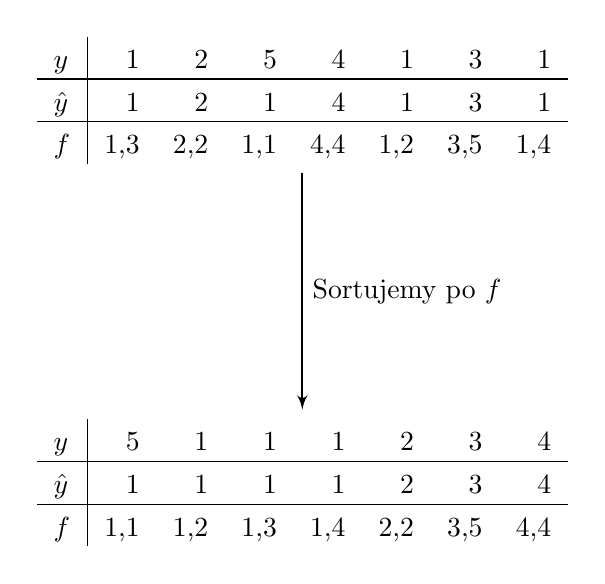
\begin{tikzpicture}
\node(gora){
\begin{tabular}{l|rrrrrrr}
 $y$ & 1 & 2 & 5 & 4 & 1 & 3 & 1\\
\hline
 $\hat{y}$ & 1 & 2 & 1 & 4 & 1 & 3 & 1\\
\hline
 $f$ & 1,3 & 2,2 & 1,1 & 4,4 & 1,2 & 3,5 & 1,4\\
\end{tabular}
};
\node[below=3cm of gora](dol){
\begin{tabular}{l|rrrrrrr}
 $y$ & 5 & 1 & 1 & 1 & 2 & 3 & 4\\
\hline
 $\hat{y}$ & 1 & 1 & 1 & 1 & 2 & 3 & 4\\
\hline
 $f$ & 1,1 & 1,2 & 1,3 & 1,4 & 2,2 & 3,5 & 4,4\\
\end{tabular}
};
\path[draw, -latex',thick](gora) -- node[midway, right] {Sortujemy po $f$} (dol);		
\end{tikzpicture}
\end{center}
\caption{Przypadek, w którym źle sklasyfikowana jest tylko jedna obserwacja. Zamiast klasy nr $5$, została przyporządkowana klasa nr $1$.\\  }
\label{vus01}
\end{subfigure}
\hspace{1cm}
\begin{subfigure}{\textwidth}
\begin{center}
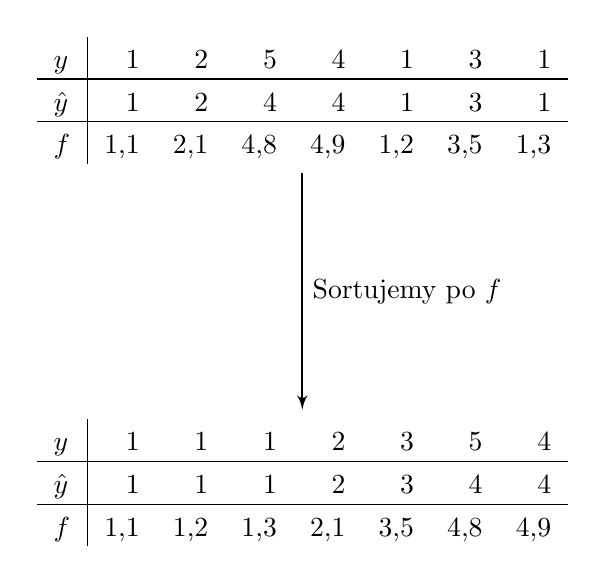
\begin{tikzpicture}
\node(gora){
\begin{tabular}{l|rrrrrrr}
 $y$ & 1 & 2 & 5 & 4 & 1 & 3 & 1\\
\hline
 $\hat{y}$ & 1 & 2 & 4 & 4 & 1 & 3 & 1\\
\hline
 $f$ & 1,1 & 2,1 & 4,8 & 4,9 & 1,2 & 3,5 & 1,3\\
\end{tabular}
};
\node[below=3cm of gora](dol){
\begin{tabular}{l|rrrrrrr}
 $y$ & 1 & 1 & 1 & 2 & 3 & 5 & 4\\
\hline
 $\hat{y}$ & 1 & 1 & 1 & 2 & 3 & 4 & 4\\
\hline
 $f$ & 1,1 & 1,2 & 1,3 & 2,1 & 3,5 & 4,8 & 4,9\\
\end{tabular}
};
\path[draw, -latex',thick](gora) -- node[midway, right] {Sortujemy po $f$} (dol);	
\end{tikzpicture}
\end{center}
\caption{Przypadek, w którym źle sklasyfikowana jest tylko jedna obserwacja. Zamiast klasy nr $5$, została przyporządkowana klasa nr $4$.}
\label{vus02}
\end{subfigure}
\caption{Tabele pokazują przykładowe zbiory testowe. W kolumnach przedstawione są kolejne obserwacje. $y$ reprezentuje prawdziwą klasę, a $\hat{y}$ klasę oszacowaną przez nas na podstawie wartości funkcji rzeczywistej $f$. Następnie, kolumny tabeli są sortowane według wartości funkcji $f$.}
\label{vusprzyklad}
\end{figure}

Załóżmy, że chcemy przyporządkować klasy pewnym obserwacjom ze zbioru testowego. Niech zbiorem klas będzie $\lbrace 1, \ldots, 5\rbrace$. Dopasowaliśmy pewien model, który działa w ten sposób, że dla danej nowej obserwacji wylicza najpierw wartość pewnej funkcji rzeczywistej $f(\cdot)$, a następnie, korzystając z pewnych progów, przyporządkowuje jej jedną z pięciu klas, w~zależności od tego, między jakimi dwoma progami znajdzie się wartość funkcji $f(\cdot)$ dla tej obserwacji. Otrzymaną w ten sposób klasę oznaczmy przez $\hat{y}$. Funkcja $f(\cdot)$ oraz wartości progów zostały nauczone podczas budowy modelu. 

Przejdźmy do omówienia przykładów. Rozważmy najpierw przypadek z Rysunku \ref{vus01}. Wszystkie klasy -- oprócz jednej -- zostały prawidłowo przyporządkowane. Podkreślmy, że pomyliliśmy się tylko w jednym przypadku. Co prawda pomyłka jest poważna (gdyż przyporządkowaliśmy klasie nr $5$ skrajnie różną wartość), ale wciąż jest to tylko jeden przypadek. Skorzystajmy ze~wzoru \eqref{dop3}, pamiętając jednocześnie, że VUS to procent dobrze uporządkowanych -- w~naszym przypadku -- piątek $(1, 2, 3, 4, 5)$ powstałych po posortowaniu wektora prawdziwych klas $y$ według rosnących wartości $f$. Bardzo łatwo zauważyć, że współczynnik VUS wyniesie~$0$. Wynika to z faktu, że jedyna odpowiedź o numerze klasy $5$ wśród zmiennej odpowiedzi uplasowała się na samym początku, tym samym uniemożliwiając znalezienie choćby jednej poprawnie uszeregowanej piątki.

Ktoś mógłby powiedzieć, że pomylenie skrajnych wartości jest poważnym błędem, więc dobrze, że VUS wyszedł taki słaby. Przyjrzyjmy się zatem przykładowi z Rysunku \ref{vus02}. Tutaj sytuacja jest podobna -- tym razem również została pomylona tylko jedna wartość (obserwacja o rzeczywistym nr 5 dostała nr 4). Błąd ten jest jednak niewielki i -- chciałoby się powiedzieć -- dopuszczalny i nieszkodliwy. Jednak w tym przypadku również nie znajdziemy ani jednej dobrze posortowanej piątki, współczynnik VUS wyniesie więc $0$.      

Podsumowując, współczynnik VUS, który ma bardzo ładną interpretację i znakomicie sprawdza się w przypadku klasyfikacji dwuetykietowej, w przypadku regresji porządkowej nie spełnia niestety swojej roli. Pozostaje nam zatem oparcie oceny klasyfikatorów jedynie na współczynnikach ACC i ABS. Nie jest to jednak satysfakcjonujące, gdyż VUS miał dawać nam pojęcie nie tyle o dokładnej poprawności klasyfikacji, ile o tym, czy obserwacje zostały poprawnie posortowane (por. Rozdział \ref{rozdz2}). Jest to aspekt bardzo istotny, gdyż tym właściwie różni się regresja porządkowa od innych rodzajów regresji czy klasyfikacji. Istnieje zatem silna potrzeba stworzenia współczynnika, który mógłby temu zadaniu sprostać. I właśnie w tym celu powstał współczynnik BSC (ang. Bubble Sorting Coefficient). 

\section{Współczynnik BSC}

Zaproponowany przeze mnie współczynnik BSC ma niemal tę samą funkcjonalność, co wskaźnik VUS. Mianowicie, pokazuje nam, w jakim stopniu nasz model prawidłowo posortował dane testowe. Jednocześnie jest on odporny na takie odchylenia danych, które automatycznie powodują wyzerowanie współczynnika VUS, a które szczegółowo omawiane były w poprzednim podrozdziale. Zyskując tę odporność, tracimy jednak na jego teoretycznej interpretacji. Bowiem o ile VUS reprezentował pewne prawdopodobieństwo (por. Rozdział \ref{rozdz2}), o tyle BSC jest tylko jego pewnym przybliżeniem. Zanim wgłębimy się jednak w jego wady i zalety, zdefiniujmy najpierw, czym właściwie ten współczynnik jest.  

\begin{algorithm}
\begin{algorithmic}
\STATE
\STATE \textbf{function} \texttt{liczba\_przestawien}$(wektor)$
\bindent
\STATE $ile\_zamian := 0$ 
\FOR {$j$ in $length(wektor):2$}
    \FOR {$i$ in $1:(j-1)$ }
        \IF {$wektor[i]>wektor[i+1]$}
            \STATE zamień $wektor[i]$ i $wektor[i+1]$
            \STATE $ile\_zamian := ile\_zamian+1$
        \ENDIF
    \ENDFOR
\ENDFOR
\eindent
\STATE \textbf{end function}
\STATE
\STATE $w1$ jest wektorem klas posortowanym ze względu na wartość funkcji $f(\cdot)$
\STATE $w2$ jest wektorem klas posortowanym malejąco
\STATE
\STATE \textbf{return} $1-(\texttt{liczba\_przestawien}(w1)/\texttt{liczba\_przestawien}(w2))$
\end{algorithmic}
\caption{Wyznaczanie współczynnika BSC}
\label{algo:bubble_sort}
\end{algorithm}

Współczynnik BSC najprościej będzie zdefiniować przy pomocy algorytmu (por. Algorytm~\ref{algo:bubble_sort}). Podobnie jak w przypadku VUS, sortujemy rzeczywiste klasy obserwacji według odpowiadających im i posortowanym rosnąco wartościom funkcji pomocniczej $f(\cdot)$. Następnie, stosując algorytm sortowania bąbelkowego, zliczamy ile przestawień sąsiednich wyrazów będzie potrzeba, by poprawnie uporządkować wejściowy wektor obserwacji. Porównujemy to do~maksymalnej liczby przestawień (czyli do takiej, która jest potrzebna do rosnącego posortowania tego samego wektora, lecz uporządkowanego malejąco, a nie według wartości funkcji $f(\cdot)$). W rezultacie otrzymujemy liczbę wahającą się od $0$, reprezentującego najgorszy przypadek, do $1$, reprezentującej przypadek najlepszy. 

Przyjrzyjmy się teraz Tabeli \ref{bsc}. Przedstawia ona $12$ przykładowych wektorów klas oraz~policzone dla nich współczynniki VUS i BSC. Łatwo zauważyć, że w większości przypadków są~one równe. Różnią się za to znacznie tam, gdzie -- wbrew intuicji -- VUS jest równy zero np. w przykładach nr $5$ i $8$, które odpowiadają tym z omawianego przez nas wcześniej Rysunku \ref{vusprzyklad}. 

\begin{table}[ht]
\centering
\begin{tabular}{rrrrrrrrrrr}
  \hline
Nr && \multicolumn{7}{c}{\parbox{4cm}{\centering\vspace{2mm}Posortowany według $f(\cdot)$ wektor prawdziwych klas\vspace{2mm}}}   & VUS [\%] & BSC [\%] \\ 
  \hline
1&&  1 &   2 &   3 &   4 &   5 &   6 &   7 & \color{red}{100,00} & \color{blue}{100.00} \\ 
2& &   1 &   1 &   1 &   2 &   3 &   4 &   5 & \color{red}{100,00} & \color{blue}{100,00} \\ 
3& &   7 &   6 &   5 &   4 &   3 &   2 &   1 & \color{red}{0,00} & \color{blue}{0,00} \\ 
4& &   5 &   4 &   3 &   2 &   1 &   1 &   1 & \color{red}{0,00} & \color{blue}{0,00} \\ 
5& &   1 &   1 &   1 &   2 &   3 &   5 &   4 & \color{red}{0,00} & \color{blue}{94,44} \\ 
6&&    5 &   1 &   1 &   1 &   2 &   3 &   4 & \color{red}{0,00} & \color{blue}{66,67} \\ 
7& &   5 &   1 &   1 &   1 &   1 &   1 &   1 & \color{red}{0,00} & \color{blue}{0,00} \\ 
8& &   5 &   1 &   1 &   1 &   1 &   1 &   6 & \color{red}{0,00} & \color{blue}{54,55} \\ 
9&&    5 &   1 &   1 &   1 &   1 &   1 &   5 & \color{red}{50,00} & \color{blue}{50,00} \\ 
10&&    1 &   1 &   1 &   5 &   1 &   1 &   1 & \color{red}{50,00} & \color{blue}{50,00} \\ 
11& &   5 &   1 &   1 &   5 &   1 &   1 &   1 & \color{red}{20,00} & \color{blue}{20,00} \\ 
12&&    1 &   5 &   2 &   3 &   4 &   5 &   4 & \color{red}{25,00} & \color{blue}{73,68} \\ 
   \hline
\end{tabular}
\caption{Porównanie wskaźników VUS i BSC}
\label{bsc}
\end{table}


Zalety współczynnika BSC są więc bardzo duże. Posiada on bowiem interpretację VUS, która jest niezwykle ważna w regresji porządkowej, a jednocześnie jest bardzo odporny na nietypowe sytuacje w danych. Szczególnie, że takie sytuacje (jak np. w przykładzie nr $5$ z Tabeli \ref{bsc}) pojawiają się bardzo często, gdy rozkład klas w danych jest nierównomierny. 

Warto jednak podkreślić, że ,,dziedzicząc'' po współczynniku VUS bardzo jasną intuicję, BSC przejmuje również niektóre jego wady. Przykładowo, gdy przyporządkujemy każdej z obserwacji klasę o jeden niższą, niż ma w rzeczywistości, wtedy zarówno VUS jak i BSC wyniosą $100\%$, gdyż wektor klas faktycznie będzie posortowany poprawnie. Jednak żadna klasa nie będzie przyporządkowana właściwie. Wadą jest również to, że i ten współczynnik stosować można jedynie do metod, które posługują się funkcją pomocniczą $f(\cdot)$ przy wyznaczaniu klasy. Jest to niejakie utrudnienie, gdyż na przykład sieci neuronowe takiej funkcji nie zwracają.

Trzeba jednak być świadomym, że w analizie wyników nie należy stosować tylko jednego współczynnika. Najbardziej skuteczne jest łączenie informacji. Warto spojrzeć zarówno na~ACC, VUS, ABS i wreszcie BSC i zastanowić się, na czym najbardziej nam zależy -- na~precyzji czy na kolejności dopasowania. Może czasem warto zrezygnować z doskonałej kolejności, by zyskać dużo większą precyzję? I odwrotnie. To już kwestia indywidualnego przypadku i charakteru naszych danych. 

\section{Dalsze wnioski}

Wróćmy do wniosków płynących z eksperymentu i jego podsumowania zawartego w Tabeli~\ref{wyniki}.

Na początku przyjrzyjmy się ostatniej kolumnie nazwanej \textit{Klasyfikacja wieloklasowa} i zaznaczonej szarym kolorem. Jako jedyna z kolumn nie odpowiada ona żadnej z metod regresji porządkowej. Jest to prosty model wielomianowy dla danych nominalnych o więcej niż dwóch klasach. Krótko mówiąc, nie uwzględnia on uporządkowania naszej zmiennej odpowiedzi. Zauważmy, że współczynnik ACC jest dla metod regresji porządkowej i klasyfikacji wieloklasowej bardzo podobny - czasem trochę mniejszy, czasem większy, ale podobny. Nasuwa się zatem pytanie, po co komplikować modele i tworzyć różne metody przeznaczone specjalnie dla regresji porządkowej, skoro zwykła i znana klasyfikacja wieloklasowa daje taki sam efekt. Odpowiedź nasuwa się sama, gdy tylko przyjrzymy się współczynnikowi BSC. Otóż w większości  przypadków jest on znacznie różny (a konkretnie znacznie mniejszy) od tego wyliczonego dla metod regresji porządkowej. Świadczy to o tym, że o ile stosując klasyfikację wieloklasową, popełniamy mniej więcej tyle samo błędów, to te błędy, które popełniamy są znacznie poważniejsze niż w pozostałych metodach (czyli przykładowo częściej mylimy skrajne wartości). Jednoznacznie potwierdza to skuteczność regresji porządkowej, która stworzona została właśnie po to, by być odporną na tego typu błędy.

Warto zwrócić również uwagę na niespodziewanie dobre zachowanie sieci neuronowych. Osiągają one najlepszy procent poprawnej klasyfikacji w $56\%$ zbiorów, a w $22\%$ niewiele odbiegają od najlepszego wyniku. Niestety nie możemy tutaj porównać współczynnika VUS ani BSC. Dlatego ryzykujemy, że uporządkowanie klas będzie słabej jakości. Trzeba jednak pamiętać, że metoda ta została specjalnie stworzona, by brać porządek klas pod uwagę, dlatego nie ma podstaw sądzić, że współczynniki te odbiegałyby bardzo od tych uzyskanych na tych samych danych dla innych metod. 

Wreszcie, widać wyraźnie, że nie ma jednej najlepszej metody. Każda ,,wygrywa" na którymś ze zbiorów oraz każda ma swoje wady i zalety. Dlatego, przeprowadzając analizę na~konkretnych danych, powinno się wziąć pod uwagę kilka istniejących sposobów modelowania, by następnie porównać je na zbiorze testowym i dopiero wtedy zadecydować, która z metod jest w naszym przypadku najlepsza. Zresztą takie podejście nie dotyczy tylko regresji porządkowej, ale wszystkich analiz statystycznych.


%%%%%%%%%%%%%%%%%%%%%%%%%%%%%%%%%%%%%%%%%%%%%%%%%%%%%%%%%%%%%%%%%%%%%%%%%%%%%%%%%%%%%%%%%%%%%%%%%%%%%%%%%%%%%%%%%%%%%%%%%%%%%

%%%%%%%%%%%%%%%%%%%%

\chapter*{Podsumowanie}

Regresja porządkowa jest ważnym działem uczenia maszynowego. Od problemu klasycznej regresji różni ją to, że zmienna odpowiedzi jest nominalna, natomiast od problemu klasyfikacji wieloklasowej to, że zmienna odpowiedzi ma pewien naturalny porządek. W mojej pracy przedstawione i omówione zostały metody modelowania regresji porządkowej opisane w dostępnej literaturze. Dodatkowo, pokazane zostały wskaźniki diagnostyczne, mające na celu ocenę jakości klasyfikatorów. Wreszcie, wszystko to zostało zebrane, porównane i podsumowane na rzeczywistych danych.

Nową rzeczą, która została przedstawiona w pracy jest współczynnik diagnostyczny BSC (ang. \textit{Bubble Sorting Coefficient}), który radzi sobie lepiej niż współczynnik VUS, zachowując jednocześnie podobną interpretację. Omówiony został dokładny algorytm jego obliczania oraz~wady i zalety samego współczynnika. 

Problem regresji porządkowej wydaje się mieć bardzo duże zastosowanie w praktyce (np.~systemy rekomendacyjne czy badania socjologiczne). Jest jednak dostępnych bardzo mało opracowań teoretycznych tego tematu, nie wspominając o oprogramowaniu. Poza tym, wciąż otwartych jest wiele zagadnień, które warto rozwijać. Przede wszystkim trzeba tu wymienić regresję porządkową, w której klasom przyporządkowane są pewne wagi. Żeby zrozumieć, o~co chodzi, odwołajmy się do przykładu ze wstępu mojej pracy, w którym chcieliśmy przewidywać opinię klienta o produkcie. Ważona regresja porządkowa zakładałaby tu, że bardziej zależy nam na poprawnym sklasyfikowaniu klientów, którym produkt potencjalnie może się spodobać niż na tych, którym może się nie spodobać (bo wtedy jest większa szansa osiągnięcia pewnych zysków) lub odwrotnie (bo wtedy nie stracimy pieniędzy na niepotrzebną reklamę). Ponadto, dalej powinno się rozwijać wskaźniki diagnostyczne, które -- jak wykazała moja praca -- nie są najlepsze. 

Problem regresji porządkowej wciąż jest zatem problemem otwartym, który prawdopodobnie bardzo mocno się w najbliższych latach rozwinie. 


%-----------------------------------------------------------------------------%

\begin{thebibliography}{9}
	
	\bibitem{fkaj} Cheng J., Source Code for Nnrank Algorithm, \url{http://sysbio.rnet.missouri.edu/multicom_toolbox/nnrank\%201.1.html}	
	
	\bibitem{nna} Cheng J., Wang Z., Pollastri G., \emph{A neural network approach to ordinal regression}, [w:]~\emph{\mbox{IEEE:} International Joint Conference on Neutral Networks}, Hong Kong 2008, str.~1279--1284	
	
	\bibitem{zbiorki} Chu W., Benchmark of ordinal regression, \url{http://www.gatsby.ucl.ac.uk/~chuwei/ordinalregression.html}	

	\bibitem{reg} Chu W., Ghahramani Z., \emph{Gaussian Processes for Ordinal Regression}, [w:] ,,Journal of~Machine Learning Research'', 2015, nr 6, str. 1019--1041	
	
	\bibitem{svm} Chu W., Sathiya Keerthi S., \emph{Support Vector Ordinal Regression}, [w:] ,,Neural Computation'', 2007, nr 19, str. 792--815 	
	
	\bibitem{af} Chu W., Source Code for Gaussian Processes for Ordinal Regression, \url{http://www.gatsby.ucl.ac.uk/~chuwei/README.gpor}	
	
	\bibitem{zbioasdgrki} Chu W., Source Code for Support Vector Ordinal Regression, \url{http://www.gatsby.ucl.ac.uk/~chuwei/svor.htm}		
	
	\bibitem{pom} Dobson A. J., \emph{An Introduction to Generalized Linear Models}, wyd. 2, Londyn 2001
	
	\bibitem{reg2} Ebden M., \emph{Gaussian Processes for Classification: A Quick Introduction}, [w:] \emph{A Gentle Introduction to Gaussian Processes. Report in three parts}, 2008	
	
	\bibitem{reg3} Ebden M., \emph{Gaussian Processes for Regression: A Quick Introduction}, [w:] \emph{A Gentle Introduction to Gaussian Processes. Report in three parts}, 2008	
	
	\bibitem{fh} Frank E., Hall M., \emph{A simple approach to ordinal classification}, [w:] \emph{Machine Learning: ECML 2001. 12th European Conference on Machine Learning. Proceedings.}, Niemcy 2001, str. 145--156

	\bibitem{koronacki} Koronacki J., Ćwik J., \emph{Statystyczne systemy uczące się}, wyd. 2, Warszawa 2008 

	\bibitem{roc2} Nakas C.T., Yiannoutsos C.T., \emph{Ordered Multiple-class ROC Analysis with continuous measurements}, [w:] ,,Statistics in Medicine'', 2004, nr 23, str. 3437--3449
		
	\bibitem{reg4} Rasmussen C., Williams C., \emph{Gaussian Processes for Machine Learning}, 2006
	
	\bibitem{zbiorki2} Torgo L., Regression Data Sets, \url{http://www.dcc.fc.up.pt/~ltorgo/Regression/DataSets.html}	
	
	\bibitem{roc1} Waegman W., De Baets B., \emph{A survey on ROC-based ordinal regression}, [w:] Fürnkranz~J., Hüllermeier E., \emph{Preference Learning}, 2010, str. 127-154
	

\end{thebibliography}

%-----------------------------------------------------------------------------%

\makestatement
\end{document}
